\documentclass{book}
\usepackage[a4paper,top=2.5cm,bottom=2.5cm,left=2.5cm,right=2.5cm]{geometry}
\usepackage{makeidx}
\usepackage{natbib}
\usepackage{graphicx}
\usepackage{multicol}
\usepackage{float}
\usepackage{listings}
\usepackage{color}
\usepackage{ifthen}
\usepackage[table]{xcolor}
\usepackage{textcomp}
\usepackage{alltt}
\usepackage{ifpdf}
\ifpdf
\usepackage[pdftex,
            pagebackref=true,
            colorlinks=true,
            linkcolor=blue,
            unicode
           ]{hyperref}
\else
\usepackage[ps2pdf,
            pagebackref=true,
            colorlinks=true,
            linkcolor=blue,
            unicode
           ]{hyperref}
\usepackage{pspicture}
\fi
\usepackage[utf8]{inputenc}
\usepackage{mathptmx}
\usepackage[scaled=.90]{helvet}
\usepackage{courier}
\usepackage{sectsty}
\usepackage{amssymb}
\usepackage[titles]{tocloft}
\usepackage{doxygen}
\lstset{language=C++,inputencoding=utf8,basicstyle=\footnotesize,breaklines=true,breakatwhitespace=true,tabsize=4,numbers=left }
\makeindex
\setcounter{tocdepth}{3}
\renewcommand{\footrulewidth}{0.4pt}
\renewcommand{\familydefault}{\sfdefault}
\hfuzz=15pt
\setlength{\emergencystretch}{15pt}
\hbadness=750
\tolerance=750
\begin{document}
\hypersetup{pageanchor=false,citecolor=blue}
\begin{titlepage}
\vspace*{7cm}
\begin{center}
{\Large Macsur Adapter }\\
\vspace*{1cm}
{\large Generated by Doxygen 1.8.3.1}\\
\vspace*{0.5cm}
{\small Tue May 14 2013 10:15:25}\\
\end{center}
\end{titlepage}
\clearemptydoublepage
\pagenumbering{roman}
\tableofcontents
\clearemptydoublepage
\pagenumbering{arabic}
\hypersetup{pageanchor=true,citecolor=blue}
\chapter{Hierarchical Index}
\section{Class Hierarchy}
This inheritance list is sorted roughly, but not completely, alphabetically\-:\begin{DoxyCompactList}
\item \contentsline{section}{Mad\-Category}{\pageref{struct_mad_category}}{}
\item Mad\-Data\-Classification\begin{DoxyCompactList}
\item \contentsline{section}{Mad\-Data\-Classification}{\pageref{class_mad_data_classification}}{}
\end{DoxyCompactList}
\item \contentsline{section}{Mad\-Guid}{\pageref{class_mad_guid}}{}
\begin{DoxyCompactList}
\item \contentsline{section}{Mad\-Data}{\pageref{class_mad_data}}{}
\item \contentsline{section}{Mad\-Model}{\pageref{class_mad_model}}{}
\end{DoxyCompactList}
\item Mad\-Main\-Window\begin{DoxyCompactList}
\item \contentsline{section}{Mad\-Main\-Window}{\pageref{class_mad_main_window}}{}
\end{DoxyCompactList}
\item \contentsline{section}{Mad\-Serialisable}{\pageref{class_mad_serialisable}}{}
\begin{DoxyCompactList}
\item \contentsline{section}{Mad\-Data}{\pageref{class_mad_data}}{}
\item \contentsline{section}{Mad\-Model}{\pageref{class_mad_model}}{}
\end{DoxyCompactList}
\item \contentsline{section}{Mad\-Sub\-Category}{\pageref{struct_mad_sub_category}}{}
\item \contentsline{section}{Mad\-Utils}{\pageref{class_mad_utils}}{}
\item Q\-Dialog\begin{DoxyCompactList}
\item \contentsline{section}{Mad\-Data\-Classification}{\pageref{class_mad_data_classification}}{}
\end{DoxyCompactList}
\item Q\-Main\-Window\begin{DoxyCompactList}
\item \contentsline{section}{Mad\-Main\-Window}{\pageref{class_mad_main_window}}{}
\end{DoxyCompactList}
\end{DoxyCompactList}

\chapter{Class Index}
\section{Class List}
Here are the classes, structs, unions and interfaces with brief descriptions\-:\begin{DoxyCompactList}
\item\contentsline{section}{\hyperlink{struct_mad_category}{Mad\-Category} }{\pageref{struct_mad_category}}{}
\item\contentsline{section}{\hyperlink{class_mad_data}{Mad\-Data} }{\pageref{class_mad_data}}{}
\item\contentsline{section}{\hyperlink{class_mad_data_classification}{Mad\-Data\-Classification} }{\pageref{class_mad_data_classification}}{}
\item\contentsline{section}{\hyperlink{class_mad_guid}{Mad\-Guid} \\*The \hyperlink{class_mad_guid}{Mad\-Guid} class An abstract base class that has a Globally Unique Identifier (G\-U\-I\-D) to represent a unique instance }{\pageref{class_mad_guid}}{}
\item\contentsline{section}{\hyperlink{class_mad_main_window}{Mad\-Main\-Window} }{\pageref{class_mad_main_window}}{}
\item\contentsline{section}{\hyperlink{class_mad_model}{Mad\-Model} \\*The \hyperlink{class_mad_model}{Mad\-Model} class, to represent a Model\-Theme }{\pageref{class_mad_model}}{}
\item\contentsline{section}{\hyperlink{class_mad_serialisable}{Mad\-Serialisable} }{\pageref{class_mad_serialisable}}{}
\item\contentsline{section}{\hyperlink{struct_mad_sub_category}{Mad\-Sub\-Category} }{\pageref{struct_mad_sub_category}}{}
\item\contentsline{section}{\hyperlink{class_mad_utils}{Mad\-Utils} }{\pageref{class_mad_utils}}{}
\end{DoxyCompactList}

\chapter{File Index}
\section{File List}
Here is a list of all files with brief descriptions\-:\begin{DoxyCompactList}
\item\contentsline{section}{/\-Users/arkygeek/\-Qt\-Projects/macsur-\/adapter/src/\-Macsur\-Adapter/\hyperlink{madmainwindow_8cpp}{madmainwindow.\-cpp} }{\pageref{madmainwindow_8cpp}}{}
\item\contentsline{section}{/\-Users/arkygeek/\-Qt\-Projects/macsur-\/adapter/src/\-Macsur\-Adapter/\hyperlink{madmainwindow_8h}{madmainwindow.\-h} }{\pageref{madmainwindow_8h}}{}
\item\contentsline{section}{/\-Users/arkygeek/\-Qt\-Projects/macsur-\/adapter/src/\-Macsur\-Adapter/\hyperlink{main_8cpp}{main.\-cpp} }{\pageref{main_8cpp}}{}
\item\contentsline{section}{/\-Users/arkygeek/\-Qt\-Projects/macsur-\/adapter/src/\-Macsur\-Adapter/gui/\hyperlink{maddataclassification_8cpp}{maddataclassification.\-cpp} }{\pageref{maddataclassification_8cpp}}{}
\item\contentsline{section}{/\-Users/arkygeek/\-Qt\-Projects/macsur-\/adapter/src/\-Macsur\-Adapter/gui/\hyperlink{maddataclassification_8h}{maddataclassification.\-h} }{\pageref{maddataclassification_8h}}{}
\item\contentsline{section}{/\-Users/arkygeek/\-Qt\-Projects/macsur-\/adapter/src/\-Macsur\-Adapter/lib/\hyperlink{mad_8h}{mad.\-h} }{\pageref{mad_8h}}{}
\item\contentsline{section}{/\-Users/arkygeek/\-Qt\-Projects/macsur-\/adapter/src/\-Macsur\-Adapter/lib/\hyperlink{maddata_8cpp}{maddata.\-cpp} }{\pageref{maddata_8cpp}}{}
\item\contentsline{section}{/\-Users/arkygeek/\-Qt\-Projects/macsur-\/adapter/src/\-Macsur\-Adapter/lib/\hyperlink{maddata_8h}{maddata.\-h} }{\pageref{maddata_8h}}{}
\item\contentsline{section}{/\-Users/arkygeek/\-Qt\-Projects/macsur-\/adapter/src/\-Macsur\-Adapter/lib/\hyperlink{madguid_8cpp}{madguid.\-cpp} }{\pageref{madguid_8cpp}}{}
\item\contentsline{section}{/\-Users/arkygeek/\-Qt\-Projects/macsur-\/adapter/src/\-Macsur\-Adapter/lib/\hyperlink{madguid_8h}{madguid.\-h} }{\pageref{madguid_8h}}{}
\item\contentsline{section}{/\-Users/arkygeek/\-Qt\-Projects/macsur-\/adapter/src/\-Macsur\-Adapter/lib/\hyperlink{madmodel_8cpp}{madmodel.\-cpp} }{\pageref{madmodel_8cpp}}{}
\item\contentsline{section}{/\-Users/arkygeek/\-Qt\-Projects/macsur-\/adapter/src/\-Macsur\-Adapter/lib/\hyperlink{madmodel_8h}{madmodel.\-h} }{\pageref{madmodel_8h}}{}
\item\contentsline{section}{/\-Users/arkygeek/\-Qt\-Projects/macsur-\/adapter/src/\-Macsur\-Adapter/lib/\hyperlink{madserialisable_8cpp}{madserialisable.\-cpp} }{\pageref{madserialisable_8cpp}}{}
\item\contentsline{section}{/\-Users/arkygeek/\-Qt\-Projects/macsur-\/adapter/src/\-Macsur\-Adapter/lib/\hyperlink{madserialisable_8h}{madserialisable.\-h} }{\pageref{madserialisable_8h}}{}
\item\contentsline{section}{/\-Users/arkygeek/\-Qt\-Projects/macsur-\/adapter/src/\-Macsur\-Adapter/lib/\hyperlink{madutils_8cpp}{madutils.\-cpp} }{\pageref{madutils_8cpp}}{}
\item\contentsline{section}{/\-Users/arkygeek/\-Qt\-Projects/macsur-\/adapter/src/\-Macsur\-Adapter/lib/\hyperlink{madutils_8h}{madutils.\-h} }{\pageref{madutils_8h}}{}
\item\contentsline{section}{/\-Users/arkygeek/\-Qt\-Projects/macsur-\/adapter/src/\-Macsur\-Adapter/lib/\hyperlink{madversion_8h}{madversion.\-h} }{\pageref{madversion_8h}}{}
\end{DoxyCompactList}

\chapter{Class Documentation}
\hypertarget{struct_mad_category}{\section{Mad\-Category Struct Reference}
\label{struct_mad_category}\index{Mad\-Category@{Mad\-Category}}
}


{\ttfamily \#include $<$maddata.\-h$>$}

\subsection*{Public Attributes}
\begin{DoxyCompactItemize}
\item 
Q\-String \hyperlink{struct_mad_category_af8fe4e8d21720e18b05210a43b2108c2}{name}
\item 
Q\-List$<$ \hyperlink{struct_mad_sub_category}{Mad\-Sub\-Category} $>$ \hyperlink{struct_mad_category_acbabe397fcbe94594e9ee0a3b8c42045}{children}
\end{DoxyCompactItemize}


\subsection{Detailed Description}


Definition at line 52 of file maddata.\-h.



\subsection{Member Data Documentation}
\hypertarget{struct_mad_category_acbabe397fcbe94594e9ee0a3b8c42045}{\index{Mad\-Category@{Mad\-Category}!children@{children}}
\index{children@{children}!MadCategory@{Mad\-Category}}
\subsubsection[{children}]{\setlength{\rightskip}{0pt plus 5cm}Q\-List$<${\bf Mad\-Sub\-Category}$>$ Mad\-Category\-::children}}\label{struct_mad_category_acbabe397fcbe94594e9ee0a3b8c42045}


Definition at line 55 of file maddata.\-h.

\hypertarget{struct_mad_category_af8fe4e8d21720e18b05210a43b2108c2}{\index{Mad\-Category@{Mad\-Category}!name@{name}}
\index{name@{name}!MadCategory@{Mad\-Category}}
\subsubsection[{name}]{\setlength{\rightskip}{0pt plus 5cm}Q\-String Mad\-Category\-::name}}\label{struct_mad_category_af8fe4e8d21720e18b05210a43b2108c2}


Definition at line 54 of file maddata.\-h.



The documentation for this struct was generated from the following file\-:\begin{DoxyCompactItemize}
\item 
/\-Users/arkygeek/\-Qt\-Projects/macsur-\/adapter/src/\-Macsur\-Adapter/lib/\hyperlink{maddata_8h}{maddata.\-h}\end{DoxyCompactItemize}

\hypertarget{class_mad_data}{\section{Mad\-Data Class Reference}
\label{class_mad_data}\index{Mad\-Data@{Mad\-Data}}
}


{\ttfamily \#include $<$maddata.\-h$>$}

Inheritance diagram for Mad\-Data\-:\begin{figure}[H]
\begin{center}
\leavevmode
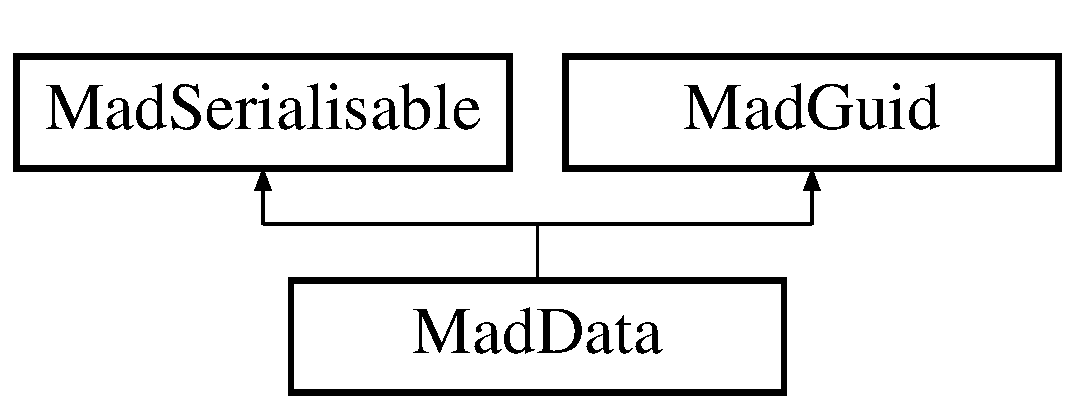
\includegraphics[height=2.000000cm]{class_mad_data}
\end{center}
\end{figure}
\subsection*{Public Member Functions}
\begin{DoxyCompactItemize}
\item 
\hyperlink{class_mad_data_a2a1f2ab4197fdfcb39dd148ad275799c}{Mad\-Data} ()
\item 
\hyperlink{class_mad_data_ad0204b1c96f0f75748e4c4c631375ce5}{Mad\-Data} (const \hyperlink{class_mad_data}{Mad\-Data} \&the\-Data)
\item 
\hyperlink{class_mad_data}{Mad\-Data} \& \hyperlink{class_mad_data_a694a4390c70108c9c55cea910dc29225}{operator=} (const \hyperlink{class_mad_data}{Mad\-Data} \&the\-Data)
\item 
Q\-String \hyperlink{class_mad_data_a83d295ac76b82edd24831a9800e275f6}{name} () const 
\item 
Q\-String \hyperlink{class_mad_data_aaf9c28a2ee3363dd2766adbbee12a890}{description} () const 
\item 
Q\-String \hyperlink{class_mad_data_a5acf4019906ad50fd96a1815b08ac11a}{image\-File} () const 
\item 
void \hyperlink{class_mad_data_af9c155374899f439660bade71c095116}{set\-Name} (Q\-String the\-Name)
\item 
void \hyperlink{class_mad_data_ac6aabfd092e0a2ce00a2f326e875946a}{set\-Description} (Q\-String the\-Description)
\item 
void \hyperlink{class_mad_data_a649da13149edf70c2a9b6273b556bd7b}{set\-Image\-File} (Q\-String the\-Image\-File\-Name)
\item 
Q\-String \hyperlink{class_mad_data_a73665b8eef0518c8c9b2df7d7565f5f8}{to\-Xml} ()
\item 
Q\-String \hyperlink{class_mad_data_a45a072ec3fee653ea15db10ab4d11156}{to\-Text} ()
\item 
Q\-String \hyperlink{class_mad_data_a985880da3130aa406964e9e8db4f0cee}{to\-Html} ()
\item 
bool \hyperlink{class_mad_data_a30677cb8685255a7939d401121525fb6}{from\-Xml} (const Q\-String the\-Xml)
\end{DoxyCompactItemize}


\subsection{Detailed Description}


Definition at line 60 of file maddata.\-h.



\subsection{Constructor \& Destructor Documentation}
\hypertarget{class_mad_data_a2a1f2ab4197fdfcb39dd148ad275799c}{\index{Mad\-Data@{Mad\-Data}!Mad\-Data@{Mad\-Data}}
\index{Mad\-Data@{Mad\-Data}!MadData@{Mad\-Data}}
\subsubsection[{Mad\-Data}]{\setlength{\rightskip}{0pt plus 5cm}Mad\-Data\-::\-Mad\-Data (
\begin{DoxyParamCaption}
{}
\end{DoxyParamCaption}
)}}\label{class_mad_data_a2a1f2ab4197fdfcb39dd148ad275799c}


Definition at line 41 of file maddata.\-cpp.

\hypertarget{class_mad_data_ad0204b1c96f0f75748e4c4c631375ce5}{\index{Mad\-Data@{Mad\-Data}!Mad\-Data@{Mad\-Data}}
\index{Mad\-Data@{Mad\-Data}!MadData@{Mad\-Data}}
\subsubsection[{Mad\-Data}]{\setlength{\rightskip}{0pt plus 5cm}Mad\-Data\-::\-Mad\-Data (
\begin{DoxyParamCaption}
\item[{const {\bf Mad\-Data} \&}]{the\-Data}
\end{DoxyParamCaption}
)}}\label{class_mad_data_ad0204b1c96f0f75748e4c4c631375ce5}
copy constructor 

Definition at line 54 of file maddata.\-cpp.



\subsection{Member Function Documentation}
\hypertarget{class_mad_data_aaf9c28a2ee3363dd2766adbbee12a890}{\index{Mad\-Data@{Mad\-Data}!description@{description}}
\index{description@{description}!MadData@{Mad\-Data}}
\subsubsection[{description}]{\setlength{\rightskip}{0pt plus 5cm}Q\-String Mad\-Data\-::description (
\begin{DoxyParamCaption}
{}
\end{DoxyParamCaption}
) const}}\label{class_mad_data_aaf9c28a2ee3363dd2766adbbee12a890}
The description of this dataset 

Definition at line 78 of file maddata.\-cpp.

\hypertarget{class_mad_data_a30677cb8685255a7939d401121525fb6}{\index{Mad\-Data@{Mad\-Data}!from\-Xml@{from\-Xml}}
\index{from\-Xml@{from\-Xml}!MadData@{Mad\-Data}}
\subsubsection[{from\-Xml}]{\setlength{\rightskip}{0pt plus 5cm}bool Mad\-Data\-::from\-Xml (
\begin{DoxyParamCaption}
\item[{const Q\-String}]{the\-Xml}
\end{DoxyParamCaption}
)\hspace{0.3cm}{\ttfamily [virtual]}}}\label{class_mad_data_a30677cb8685255a7939d401121525fb6}
Read this object from xml and return result as true for success, false for failure. \begin{DoxySeeAlso}{See Also}
\hyperlink{class_mad_serialisable}{Mad\-Serialisable}  this class inherits the serialisable interface so it M\-U\-S\-T implement this 
\end{DoxySeeAlso}


Implements \hyperlink{class_mad_serialisable_a37d5fc3b08cddd05c4ddffdf3fd43535}{Mad\-Serialisable}.



Definition at line 105 of file maddata.\-cpp.

\hypertarget{class_mad_data_a5acf4019906ad50fd96a1815b08ac11a}{\index{Mad\-Data@{Mad\-Data}!image\-File@{image\-File}}
\index{image\-File@{image\-File}!MadData@{Mad\-Data}}
\subsubsection[{image\-File}]{\setlength{\rightskip}{0pt plus 5cm}Q\-String Mad\-Data\-::image\-File (
\begin{DoxyParamCaption}
{}
\end{DoxyParamCaption}
) const}}\label{class_mad_data_a5acf4019906ad50fd96a1815b08ac11a}
The cultivation vars of this dataset The image file associated with the dataset 

Definition at line 83 of file maddata.\-cpp.

\hypertarget{class_mad_data_a83d295ac76b82edd24831a9800e275f6}{\index{Mad\-Data@{Mad\-Data}!name@{name}}
\index{name@{name}!MadData@{Mad\-Data}}
\subsubsection[{name}]{\setlength{\rightskip}{0pt plus 5cm}Q\-String Mad\-Data\-::name (
\begin{DoxyParamCaption}
{}
\end{DoxyParamCaption}
) const}}\label{class_mad_data_a83d295ac76b82edd24831a9800e275f6}
The name of this dataset 

Definition at line 73 of file maddata.\-cpp.

\hypertarget{class_mad_data_a694a4390c70108c9c55cea910dc29225}{\index{Mad\-Data@{Mad\-Data}!operator=@{operator=}}
\index{operator=@{operator=}!MadData@{Mad\-Data}}
\subsubsection[{operator=}]{\setlength{\rightskip}{0pt plus 5cm}{\bf Mad\-Data} \& Mad\-Data\-::operator= (
\begin{DoxyParamCaption}
\item[{const {\bf Mad\-Data} \&}]{the\-Data}
\end{DoxyParamCaption}
)}}\label{class_mad_data_a694a4390c70108c9c55cea910dc29225}
Assignement operator 

Definition at line 62 of file maddata.\-cpp.

\hypertarget{class_mad_data_ac6aabfd092e0a2ce00a2f326e875946a}{\index{Mad\-Data@{Mad\-Data}!set\-Description@{set\-Description}}
\index{set\-Description@{set\-Description}!MadData@{Mad\-Data}}
\subsubsection[{set\-Description}]{\setlength{\rightskip}{0pt plus 5cm}void Mad\-Data\-::set\-Description (
\begin{DoxyParamCaption}
\item[{Q\-String}]{the\-Description}
\end{DoxyParamCaption}
)}}\label{class_mad_data_ac6aabfd092e0a2ce00a2f326e875946a}
Set the model description \begin{DoxySeeAlso}{See Also}
\hyperlink{class_mad_data_aaf9c28a2ee3363dd2766adbbee12a890}{description()} 
\end{DoxySeeAlso}


Definition at line 95 of file maddata.\-cpp.

\hypertarget{class_mad_data_a649da13149edf70c2a9b6273b556bd7b}{\index{Mad\-Data@{Mad\-Data}!set\-Image\-File@{set\-Image\-File}}
\index{set\-Image\-File@{set\-Image\-File}!MadData@{Mad\-Data}}
\subsubsection[{set\-Image\-File}]{\setlength{\rightskip}{0pt plus 5cm}void Mad\-Data\-::set\-Image\-File (
\begin{DoxyParamCaption}
\item[{Q\-String}]{the\-Image\-File\-Name}
\end{DoxyParamCaption}
)}}\label{class_mad_data_a649da13149edf70c2a9b6273b556bd7b}
Set the image file \begin{DoxySeeAlso}{See Also}
\hyperlink{class_mad_data_a5acf4019906ad50fd96a1815b08ac11a}{image\-File()} 
\end{DoxySeeAlso}


Definition at line 100 of file maddata.\-cpp.

\hypertarget{class_mad_data_af9c155374899f439660bade71c095116}{\index{Mad\-Data@{Mad\-Data}!set\-Name@{set\-Name}}
\index{set\-Name@{set\-Name}!MadData@{Mad\-Data}}
\subsubsection[{set\-Name}]{\setlength{\rightskip}{0pt plus 5cm}void Mad\-Data\-::set\-Name (
\begin{DoxyParamCaption}
\item[{Q\-String}]{the\-Name}
\end{DoxyParamCaption}
)}}\label{class_mad_data_af9c155374899f439660bade71c095116}
Set the model\-Name \begin{DoxySeeAlso}{See Also}
\hyperlink{class_mad_data_a83d295ac76b82edd24831a9800e275f6}{name()} 
\end{DoxySeeAlso}


Definition at line 90 of file maddata.\-cpp.

\hypertarget{class_mad_data_a985880da3130aa406964e9e8db4f0cee}{\index{Mad\-Data@{Mad\-Data}!to\-Html@{to\-Html}}
\index{to\-Html@{to\-Html}!MadData@{Mad\-Data}}
\subsubsection[{to\-Html}]{\setlength{\rightskip}{0pt plus 5cm}Q\-String Mad\-Data\-::to\-Html (
\begin{DoxyParamCaption}
{}
\end{DoxyParamCaption}
)}}\label{class_mad_data_a985880da3130aa406964e9e8db4f0cee}
Return a html text representation of this layer 

Definition at line 155 of file maddata.\-cpp.

\hypertarget{class_mad_data_a45a072ec3fee653ea15db10ab4d11156}{\index{Mad\-Data@{Mad\-Data}!to\-Text@{to\-Text}}
\index{to\-Text@{to\-Text}!MadData@{Mad\-Data}}
\subsubsection[{to\-Text}]{\setlength{\rightskip}{0pt plus 5cm}Q\-String Mad\-Data\-::to\-Text (
\begin{DoxyParamCaption}
{}
\end{DoxyParamCaption}
)}}\label{class_mad_data_a45a072ec3fee653ea15db10ab4d11156}
Return a plain text representation of this layer 

Definition at line 146 of file maddata.\-cpp.

\hypertarget{class_mad_data_a73665b8eef0518c8c9b2df7d7565f5f8}{\index{Mad\-Data@{Mad\-Data}!to\-Xml@{to\-Xml}}
\index{to\-Xml@{to\-Xml}!MadData@{Mad\-Data}}
\subsubsection[{to\-Xml}]{\setlength{\rightskip}{0pt plus 5cm}Q\-String Mad\-Data\-::to\-Xml (
\begin{DoxyParamCaption}
{}
\end{DoxyParamCaption}
)\hspace{0.3cm}{\ttfamily [virtual]}}}\label{class_mad_data_a73665b8eef0518c8c9b2df7d7565f5f8}
Return an xml representation of this layer  this class inherits the serialisable interface so it M\-U\-S\-T implement this 

Implements \hyperlink{class_mad_serialisable_ad54654484660b5b0391f5e8765070ec8}{Mad\-Serialisable}.



Definition at line 124 of file maddata.\-cpp.



The documentation for this class was generated from the following files\-:\begin{DoxyCompactItemize}
\item 
/\-Users/arkygeek/\-Qt\-Projects/macsur-\/adapter/src/\-Macsur\-Adapter/lib/\hyperlink{maddata_8h}{maddata.\-h}\item 
/\-Users/arkygeek/\-Qt\-Projects/macsur-\/adapter/src/\-Macsur\-Adapter/lib/\hyperlink{maddata_8cpp}{maddata.\-cpp}\end{DoxyCompactItemize}

\hypertarget{class_mad_data_classification}{\section{Mad\-Data\-Classification Class Reference}
\label{class_mad_data_classification}\index{Mad\-Data\-Classification@{Mad\-Data\-Classification}}
}


{\ttfamily \#include $<$maddataclassification.\-h$>$}

Inheritance diagram for Mad\-Data\-Classification\-:\begin{figure}[H]
\begin{center}
\leavevmode
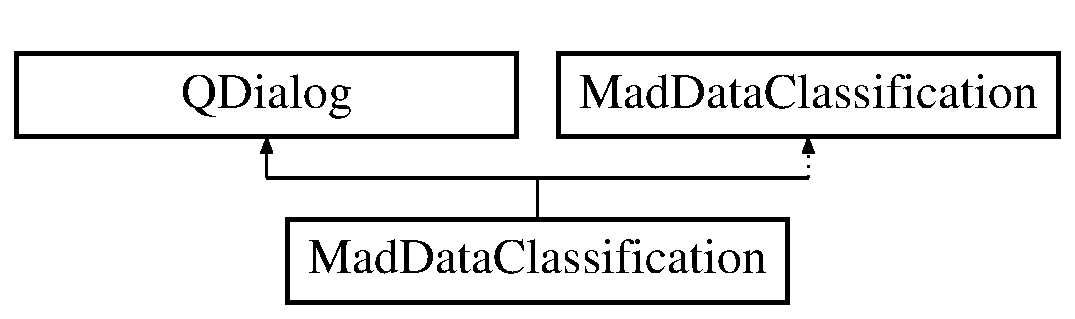
\includegraphics[height=2.000000cm]{class_mad_data_classification}
\end{center}
\end{figure}
\subsection*{Public Member Functions}
\begin{DoxyCompactItemize}
\item 
\hyperlink{class_mad_data_classification_a8c1d8f63b5d348531fbccb263f7f0635}{Mad\-Data\-Classification} (Q\-Widget $\ast$parent=0)
\end{DoxyCompactItemize}
\subsection*{Protected Member Functions}
\begin{DoxyCompactItemize}
\item 
void \hyperlink{class_mad_data_classification_a75376b6826fe8316fc1e5517111defb4}{change\-Event} (Q\-Event $\ast$e)
\end{DoxyCompactItemize}


\subsection{Detailed Description}


Definition at line 27 of file maddataclassification.\-h.



\subsection{Constructor \& Destructor Documentation}
\hypertarget{class_mad_data_classification_a8c1d8f63b5d348531fbccb263f7f0635}{\index{Mad\-Data\-Classification@{Mad\-Data\-Classification}!Mad\-Data\-Classification@{Mad\-Data\-Classification}}
\index{Mad\-Data\-Classification@{Mad\-Data\-Classification}!MadDataClassification@{Mad\-Data\-Classification}}
\subsubsection[{Mad\-Data\-Classification}]{\setlength{\rightskip}{0pt plus 5cm}Mad\-Data\-Classification\-::\-Mad\-Data\-Classification (
\begin{DoxyParamCaption}
\item[{Q\-Widget $\ast$}]{parent = {\ttfamily 0}}
\end{DoxyParamCaption}
)\hspace{0.3cm}{\ttfamily [explicit]}}}\label{class_mad_data_classification_a8c1d8f63b5d348531fbccb263f7f0635}


Definition at line 29 of file maddataclassification.\-cpp.



\subsection{Member Function Documentation}
\hypertarget{class_mad_data_classification_a75376b6826fe8316fc1e5517111defb4}{\index{Mad\-Data\-Classification@{Mad\-Data\-Classification}!change\-Event@{change\-Event}}
\index{change\-Event@{change\-Event}!MadDataClassification@{Mad\-Data\-Classification}}
\subsubsection[{change\-Event}]{\setlength{\rightskip}{0pt plus 5cm}void Mad\-Data\-Classification\-::change\-Event (
\begin{DoxyParamCaption}
\item[{Q\-Event $\ast$}]{e}
\end{DoxyParamCaption}
)\hspace{0.3cm}{\ttfamily [protected]}}}\label{class_mad_data_classification_a75376b6826fe8316fc1e5517111defb4}


Definition at line 39 of file maddataclassification.\-cpp.



The documentation for this class was generated from the following files\-:\begin{DoxyCompactItemize}
\item 
/\-Users/arkygeek/\-Qt\-Projects/macsur-\/adapter/src/\-Macsur\-Adapter/gui/\hyperlink{maddataclassification_8h}{maddataclassification.\-h}\item 
/\-Users/arkygeek/\-Qt\-Projects/macsur-\/adapter/src/\-Macsur\-Adapter/gui/\hyperlink{maddataclassification_8cpp}{maddataclassification.\-cpp}\end{DoxyCompactItemize}

\hypertarget{class_mad_guid}{\section{Mad\-Guid Class Reference}
\label{class_mad_guid}\index{Mad\-Guid@{Mad\-Guid}}
}


The \hyperlink{class_mad_guid}{Mad\-Guid} class An abstract base class that has a Globally Unique Identifier (G\-U\-I\-D) to represent a unique instance.  




{\ttfamily \#include $<$madguid.\-h$>$}

Inheritance diagram for Mad\-Guid\-:\begin{figure}[H]
\begin{center}
\leavevmode
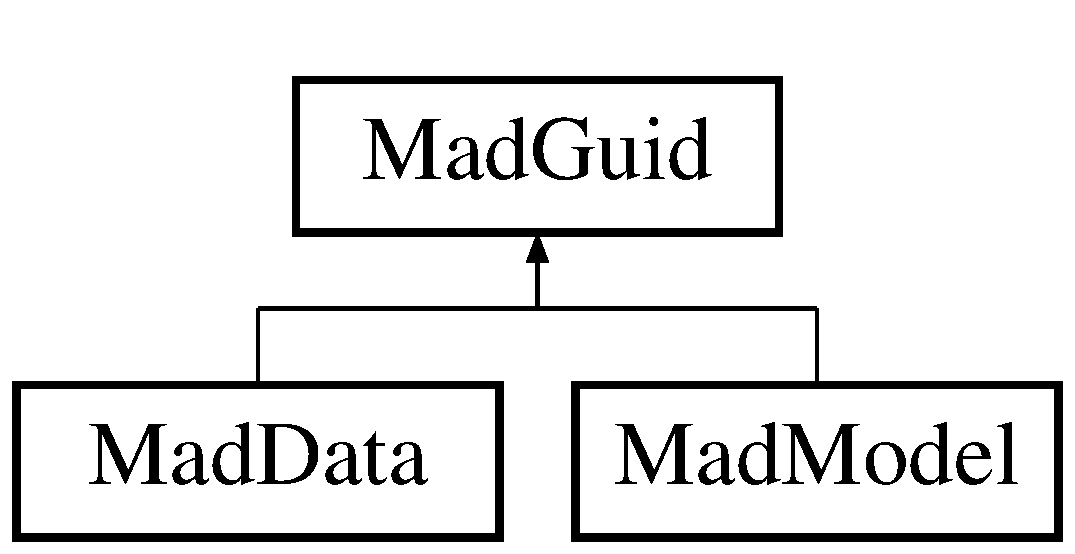
\includegraphics[height=2.000000cm]{class_mad_guid}
\end{center}
\end{figure}
\subsection*{Public Member Functions}
\begin{DoxyCompactItemize}
\item 
\hyperlink{class_mad_guid_a119759ea390708eab3df016639b01cc7}{Mad\-Guid} ()
\item 
Q\-String \hyperlink{class_mad_guid_abd5fd246f0be83f0b9572363a78f66be}{guid} () const 
\begin{DoxyCompactList}\small\item\em \hyperlink{class_mad_guid_abd5fd246f0be83f0b9572363a78f66be}{Mad\-Guid\-::guid}. \end{DoxyCompactList}\item 
void \hyperlink{class_mad_guid_a899833db4b57903608571b737baa5a0a}{set\-Guid} (Q\-String the\-Guid=\char`\"{}\char`\"{})
\begin{DoxyCompactList}\small\item\em \hyperlink{class_mad_guid_a899833db4b57903608571b737baa5a0a}{Mad\-Guid\-::set\-Guid}. \end{DoxyCompactList}\end{DoxyCompactItemize}


\subsection{Detailed Description}
The \hyperlink{class_mad_guid}{Mad\-Guid} class An abstract base class that has a Globally Unique Identifier (G\-U\-I\-D) to represent a unique instance. 

Definition at line 32 of file madguid.\-h.



\subsection{Constructor \& Destructor Documentation}
\hypertarget{class_mad_guid_a119759ea390708eab3df016639b01cc7}{\index{Mad\-Guid@{Mad\-Guid}!Mad\-Guid@{Mad\-Guid}}
\index{Mad\-Guid@{Mad\-Guid}!MadGuid@{Mad\-Guid}}
\subsubsection[{Mad\-Guid}]{\setlength{\rightskip}{0pt plus 5cm}Mad\-Guid\-::\-Mad\-Guid (
\begin{DoxyParamCaption}
{}
\end{DoxyParamCaption}
)}}\label{class_mad_guid_a119759ea390708eab3df016639b01cc7}
Constructor 

Definition at line 28 of file madguid.\-cpp.



\subsection{Member Function Documentation}
\hypertarget{class_mad_guid_abd5fd246f0be83f0b9572363a78f66be}{\index{Mad\-Guid@{Mad\-Guid}!guid@{guid}}
\index{guid@{guid}!MadGuid@{Mad\-Guid}}
\subsubsection[{guid}]{\setlength{\rightskip}{0pt plus 5cm}Q\-String Mad\-Guid\-::guid (
\begin{DoxyParamCaption}
{}
\end{DoxyParamCaption}
) const}}\label{class_mad_guid_abd5fd246f0be83f0b9572363a78f66be}


\hyperlink{class_mad_guid_abd5fd246f0be83f0b9572363a78f66be}{Mad\-Guid\-::guid}. 

Destructor Retrieve the G\-U\-I\-D

\begin{DoxyReturn}{Returns}

\end{DoxyReturn}


Definition at line 40 of file madguid.\-cpp.

\hypertarget{class_mad_guid_a899833db4b57903608571b737baa5a0a}{\index{Mad\-Guid@{Mad\-Guid}!set\-Guid@{set\-Guid}}
\index{set\-Guid@{set\-Guid}!MadGuid@{Mad\-Guid}}
\subsubsection[{set\-Guid}]{\setlength{\rightskip}{0pt plus 5cm}void Mad\-Guid\-::set\-Guid (
\begin{DoxyParamCaption}
\item[{Q\-String}]{the\-Guid = {\ttfamily \char`\"{}\char`\"{}}}
\end{DoxyParamCaption}
)}}\label{class_mad_guid_a899833db4b57903608571b737baa5a0a}


\hyperlink{class_mad_guid_a899833db4b57903608571b737baa5a0a}{Mad\-Guid\-::set\-Guid}. 


\begin{DoxyParams}{Parameters}
{\em the\-Guid} & \\
\hline
\end{DoxyParams}


Definition at line 49 of file madguid.\-cpp.



The documentation for this class was generated from the following files\-:\begin{DoxyCompactItemize}
\item 
/\-Users/arkygeek/\-Qt\-Projects/macsur-\/adapter/src/\-Macsur\-Adapter/lib/\hyperlink{madguid_8h}{madguid.\-h}\item 
/\-Users/arkygeek/\-Qt\-Projects/macsur-\/adapter/src/\-Macsur\-Adapter/lib/\hyperlink{madguid_8cpp}{madguid.\-cpp}\end{DoxyCompactItemize}

\hypertarget{class_mad_main_window}{\section{Mad\-Main\-Window Class Reference}
\label{class_mad_main_window}\index{Mad\-Main\-Window@{Mad\-Main\-Window}}
}


{\ttfamily \#include $<$madmainwindow.\-h$>$}

Inheritance diagram for Mad\-Main\-Window\-:\begin{figure}[H]
\begin{center}
\leavevmode
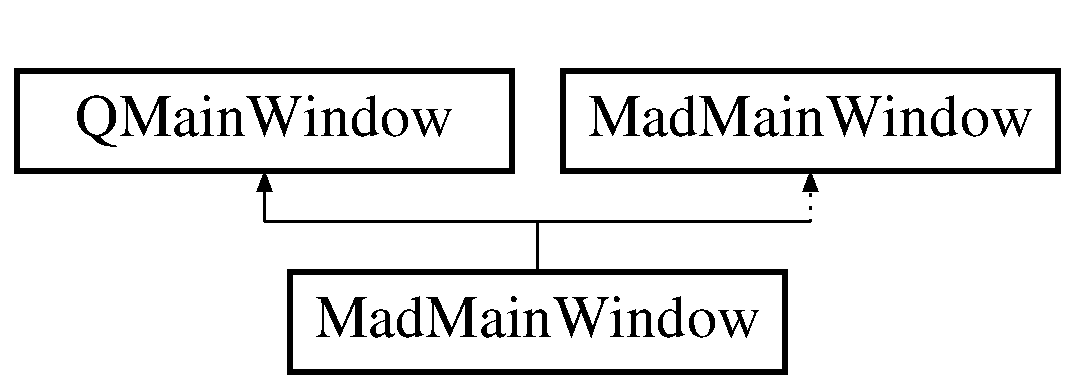
\includegraphics[height=2.000000cm]{class_mad_main_window}
\end{center}
\end{figure}
\subsection*{Public Member Functions}
\begin{DoxyCompactItemize}
\item 
\hyperlink{class_mad_main_window_adb4f90643637c6d6f89fb77c25ced55b}{Mad\-Main\-Window} (Q\-Widget $\ast$parent=0)
\end{DoxyCompactItemize}
\subsection*{Protected Member Functions}
\begin{DoxyCompactItemize}
\item 
void \hyperlink{class_mad_main_window_af9c57e0984b87146a1de895bc1a5b54b}{change\-Event} (Q\-Event $\ast$e)
\begin{DoxyCompactList}\small\item\em load\-Models Refreshes the list of known models \end{DoxyCompactList}\end{DoxyCompactItemize}


\subsection{Detailed Description}
This is the main G\-U\-I class \begin{DoxyAuthor}{Author}
Jason Jorgenson 
\end{DoxyAuthor}


Definition at line 38 of file madmainwindow.\-h.



\subsection{Constructor \& Destructor Documentation}
\hypertarget{class_mad_main_window_adb4f90643637c6d6f89fb77c25ced55b}{\index{Mad\-Main\-Window@{Mad\-Main\-Window}!Mad\-Main\-Window@{Mad\-Main\-Window}}
\index{Mad\-Main\-Window@{Mad\-Main\-Window}!MadMainWindow@{Mad\-Main\-Window}}
\subsubsection[{Mad\-Main\-Window}]{\setlength{\rightskip}{0pt plus 5cm}Mad\-Main\-Window\-::\-Mad\-Main\-Window (
\begin{DoxyParamCaption}
\item[{Q\-Widget $\ast$}]{parent = {\ttfamily 0}}
\end{DoxyParamCaption}
)\hspace{0.3cm}{\ttfamily [explicit]}}}\label{class_mad_main_window_adb4f90643637c6d6f89fb77c25ced55b}
This is the main form G\-U\-I of M\-A\-D (Macsur A\-Dapter) It sets up the required slot connections and initialises the G\-U\-I 
\begin{DoxyParams}{Parameters}
{\em parent} & \\
\hline
\end{DoxyParams}


Definition at line 31 of file madmainwindow.\-cpp.



\subsection{Member Function Documentation}
\hypertarget{class_mad_main_window_af9c57e0984b87146a1de895bc1a5b54b}{\index{Mad\-Main\-Window@{Mad\-Main\-Window}!change\-Event@{change\-Event}}
\index{change\-Event@{change\-Event}!MadMainWindow@{Mad\-Main\-Window}}
\subsubsection[{change\-Event}]{\setlength{\rightskip}{0pt plus 5cm}void Mad\-Main\-Window\-::change\-Event (
\begin{DoxyParamCaption}
\item[{Q\-Event $\ast$}]{e}
\end{DoxyParamCaption}
)\hspace{0.3cm}{\ttfamily [protected]}}}\label{class_mad_main_window_af9c57e0984b87146a1de895bc1a5b54b}


load\-Models Refreshes the list of known models 

change\-Event for translations in the future 
\begin{DoxyParams}{Parameters}
{\em e} & \\
\hline
\end{DoxyParams}


Definition at line 44 of file madmainwindow.\-cpp.



The documentation for this class was generated from the following files\-:\begin{DoxyCompactItemize}
\item 
/\-Users/arkygeek/\-Qt\-Projects/macsur-\/adapter/src/\-Macsur\-Adapter/\hyperlink{madmainwindow_8h}{madmainwindow.\-h}\item 
/\-Users/arkygeek/\-Qt\-Projects/macsur-\/adapter/src/\-Macsur\-Adapter/\hyperlink{madmainwindow_8cpp}{madmainwindow.\-cpp}\end{DoxyCompactItemize}

\hypertarget{class_mad_model}{\section{Mad\-Model Class Reference}
\label{class_mad_model}\index{Mad\-Model@{Mad\-Model}}
}


The \hyperlink{class_mad_model}{Mad\-Model} class, to represent a Model\-Theme.  




{\ttfamily \#include $<$madmodel.\-h$>$}

Inheritance diagram for Mad\-Model\-:\begin{figure}[H]
\begin{center}
\leavevmode
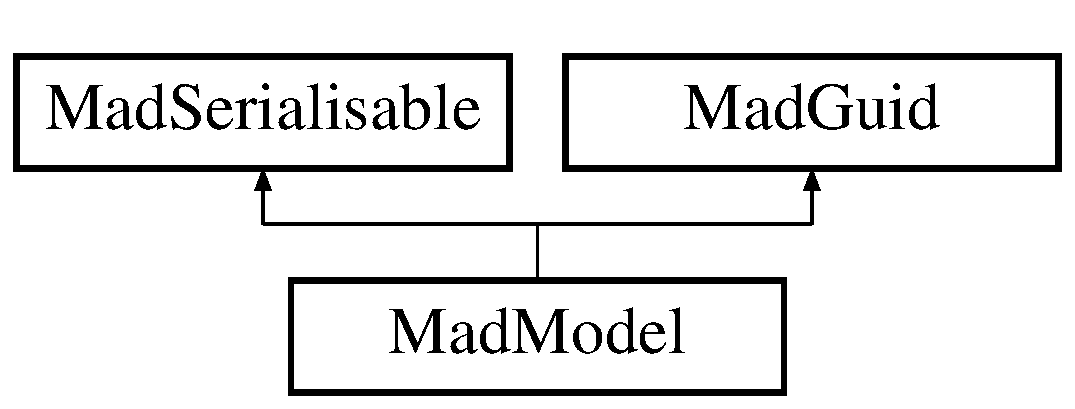
\includegraphics[height=2.000000cm]{class_mad_model}
\end{center}
\end{figure}
\subsection*{Public Member Functions}
\begin{DoxyCompactItemize}
\item 
\hyperlink{class_mad_model_af27ca3c9c638a960822924193786d0e9}{Mad\-Model} ()
\item 
\hyperlink{class_mad_model_af8cf7ab044805122243b9153cc56e733}{Mad\-Model} (const \hyperlink{class_mad_model}{Mad\-Model} \&the\-Model)
\item 
\hyperlink{class_mad_model}{Mad\-Model} \& \hyperlink{class_mad_model_a8c064230a0f61bafb7a546a565934585}{operator=} (const \hyperlink{class_mad_model}{Mad\-Model} \&the\-Model)
\item 
Q\-String \hyperlink{class_mad_model_aaad4ceb50f8a4422582c712050469fd7}{name} () const 
\item 
Q\-String \hyperlink{class_mad_model_a424649185054ab1c5e09ce1b7f14bd3b}{description} () const 
\item 
Q\-String \hyperlink{class_mad_model_abd250700ecd6b39bb105bd4700df7026}{image\-File} () const 
\item 
void \hyperlink{class_mad_model_a6fb035d7103acd537ba1e1e2ca61e1e3}{set\-Name} (Q\-String the\-Name)
\item 
void \hyperlink{class_mad_model_afe66211bf0ca450f9bf80556bf54968a}{set\-Description} (Q\-String the\-Description)
\item 
void \hyperlink{class_mad_model_a138bc5e80dda34e870183f7c016c565a}{set\-Image\-File} (Q\-String the\-Image\-File\-Name)
\item 
Q\-String \hyperlink{class_mad_model_a797ce6bb5f6f2798640ef505ed1ee644}{to\-Xml} ()
\item 
Q\-String \hyperlink{class_mad_model_a9fcc10c120e3ee0d947be19fe3e023e5}{to\-Text} ()
\item 
Q\-String \hyperlink{class_mad_model_a45492403d449bbd9dea4e9c567591687}{to\-Html} ()
\item 
bool \hyperlink{class_mad_model_ada33c0eed39499b58d0a886566732607}{from\-Xml} (const Q\-String the\-Xml)
\end{DoxyCompactItemize}


\subsection{Detailed Description}
The \hyperlink{class_mad_model}{Mad\-Model} class, to represent a Model\-Theme. 

Definition at line 56 of file madmodel.\-h.



\subsection{Constructor \& Destructor Documentation}
\hypertarget{class_mad_model_af27ca3c9c638a960822924193786d0e9}{\index{Mad\-Model@{Mad\-Model}!Mad\-Model@{Mad\-Model}}
\index{Mad\-Model@{Mad\-Model}!MadModel@{Mad\-Model}}
\subsubsection[{Mad\-Model}]{\setlength{\rightskip}{0pt plus 5cm}Mad\-Model\-::\-Mad\-Model (
\begin{DoxyParamCaption}
{}
\end{DoxyParamCaption}
)}}\label{class_mad_model_af27ca3c9c638a960822924193786d0e9}
Constructor . 

Definition at line 33 of file madmodel.\-cpp.

\hypertarget{class_mad_model_af8cf7ab044805122243b9153cc56e733}{\index{Mad\-Model@{Mad\-Model}!Mad\-Model@{Mad\-Model}}
\index{Mad\-Model@{Mad\-Model}!MadModel@{Mad\-Model}}
\subsubsection[{Mad\-Model}]{\setlength{\rightskip}{0pt plus 5cm}Mad\-Model\-::\-Mad\-Model (
\begin{DoxyParamCaption}
\item[{const {\bf Mad\-Model} \&}]{the\-Model}
\end{DoxyParamCaption}
)}}\label{class_mad_model_af8cf7ab044805122243b9153cc56e733}
Destructor . copy constructor 

Definition at line 46 of file madmodel.\-cpp.



\subsection{Member Function Documentation}
\hypertarget{class_mad_model_a424649185054ab1c5e09ce1b7f14bd3b}{\index{Mad\-Model@{Mad\-Model}!description@{description}}
\index{description@{description}!MadModel@{Mad\-Model}}
\subsubsection[{description}]{\setlength{\rightskip}{0pt plus 5cm}Q\-String Mad\-Model\-::description (
\begin{DoxyParamCaption}
{}
\end{DoxyParamCaption}
) const}}\label{class_mad_model_a424649185054ab1c5e09ce1b7f14bd3b}
The description of this model 

Definition at line 70 of file madmodel.\-cpp.

\hypertarget{class_mad_model_ada33c0eed39499b58d0a886566732607}{\index{Mad\-Model@{Mad\-Model}!from\-Xml@{from\-Xml}}
\index{from\-Xml@{from\-Xml}!MadModel@{Mad\-Model}}
\subsubsection[{from\-Xml}]{\setlength{\rightskip}{0pt plus 5cm}bool Mad\-Model\-::from\-Xml (
\begin{DoxyParamCaption}
\item[{const Q\-String}]{the\-Xml}
\end{DoxyParamCaption}
)\hspace{0.3cm}{\ttfamily [virtual]}}}\label{class_mad_model_ada33c0eed39499b58d0a886566732607}
Read this object from xml and return result as true for success, false for failure. \begin{DoxySeeAlso}{See Also}
\hyperlink{class_mad_serialisable}{Mad\-Serialisable}  this class inherits the serialisable interface so it M\-U\-S\-T implement this 
\end{DoxySeeAlso}


Implements \hyperlink{class_mad_serialisable_a37d5fc3b08cddd05c4ddffdf3fd43535}{Mad\-Serialisable}.



Definition at line 97 of file madmodel.\-cpp.

\hypertarget{class_mad_model_abd250700ecd6b39bb105bd4700df7026}{\index{Mad\-Model@{Mad\-Model}!image\-File@{image\-File}}
\index{image\-File@{image\-File}!MadModel@{Mad\-Model}}
\subsubsection[{image\-File}]{\setlength{\rightskip}{0pt plus 5cm}Q\-String Mad\-Model\-::image\-File (
\begin{DoxyParamCaption}
{}
\end{DoxyParamCaption}
) const}}\label{class_mad_model_abd250700ecd6b39bb105bd4700df7026}
The image file associated with the model 

Definition at line 75 of file madmodel.\-cpp.

\hypertarget{class_mad_model_aaad4ceb50f8a4422582c712050469fd7}{\index{Mad\-Model@{Mad\-Model}!name@{name}}
\index{name@{name}!MadModel@{Mad\-Model}}
\subsubsection[{name}]{\setlength{\rightskip}{0pt plus 5cm}Q\-String Mad\-Model\-::name (
\begin{DoxyParamCaption}
{}
\end{DoxyParamCaption}
) const}}\label{class_mad_model_aaad4ceb50f8a4422582c712050469fd7}
The name of this model 

Definition at line 65 of file madmodel.\-cpp.

\hypertarget{class_mad_model_a8c064230a0f61bafb7a546a565934585}{\index{Mad\-Model@{Mad\-Model}!operator=@{operator=}}
\index{operator=@{operator=}!MadModel@{Mad\-Model}}
\subsubsection[{operator=}]{\setlength{\rightskip}{0pt plus 5cm}{\bf Mad\-Model} \& Mad\-Model\-::operator= (
\begin{DoxyParamCaption}
\item[{const {\bf Mad\-Model} \&}]{the\-Model}
\end{DoxyParamCaption}
)}}\label{class_mad_model_a8c064230a0f61bafb7a546a565934585}
Assignement operator 

Definition at line 54 of file madmodel.\-cpp.

\hypertarget{class_mad_model_afe66211bf0ca450f9bf80556bf54968a}{\index{Mad\-Model@{Mad\-Model}!set\-Description@{set\-Description}}
\index{set\-Description@{set\-Description}!MadModel@{Mad\-Model}}
\subsubsection[{set\-Description}]{\setlength{\rightskip}{0pt plus 5cm}void Mad\-Model\-::set\-Description (
\begin{DoxyParamCaption}
\item[{Q\-String}]{the\-Description}
\end{DoxyParamCaption}
)}}\label{class_mad_model_afe66211bf0ca450f9bf80556bf54968a}
Set the model description \begin{DoxySeeAlso}{See Also}
\hyperlink{class_mad_model_a424649185054ab1c5e09ce1b7f14bd3b}{description()} 
\end{DoxySeeAlso}


Definition at line 87 of file madmodel.\-cpp.

\hypertarget{class_mad_model_a138bc5e80dda34e870183f7c016c565a}{\index{Mad\-Model@{Mad\-Model}!set\-Image\-File@{set\-Image\-File}}
\index{set\-Image\-File@{set\-Image\-File}!MadModel@{Mad\-Model}}
\subsubsection[{set\-Image\-File}]{\setlength{\rightskip}{0pt plus 5cm}void Mad\-Model\-::set\-Image\-File (
\begin{DoxyParamCaption}
\item[{Q\-String}]{the\-Image\-File\-Name}
\end{DoxyParamCaption}
)}}\label{class_mad_model_a138bc5e80dda34e870183f7c016c565a}
Set the image file \begin{DoxySeeAlso}{See Also}
\hyperlink{class_mad_model_abd250700ecd6b39bb105bd4700df7026}{image\-File()} 
\end{DoxySeeAlso}


Definition at line 92 of file madmodel.\-cpp.

\hypertarget{class_mad_model_a6fb035d7103acd537ba1e1e2ca61e1e3}{\index{Mad\-Model@{Mad\-Model}!set\-Name@{set\-Name}}
\index{set\-Name@{set\-Name}!MadModel@{Mad\-Model}}
\subsubsection[{set\-Name}]{\setlength{\rightskip}{0pt plus 5cm}void Mad\-Model\-::set\-Name (
\begin{DoxyParamCaption}
\item[{Q\-String}]{the\-Name}
\end{DoxyParamCaption}
)}}\label{class_mad_model_a6fb035d7103acd537ba1e1e2ca61e1e3}
Set the model\-Name \begin{DoxySeeAlso}{See Also}
\hyperlink{class_mad_model_aaad4ceb50f8a4422582c712050469fd7}{name()} 
\end{DoxySeeAlso}


Definition at line 82 of file madmodel.\-cpp.

\hypertarget{class_mad_model_a45492403d449bbd9dea4e9c567591687}{\index{Mad\-Model@{Mad\-Model}!to\-Html@{to\-Html}}
\index{to\-Html@{to\-Html}!MadModel@{Mad\-Model}}
\subsubsection[{to\-Html}]{\setlength{\rightskip}{0pt plus 5cm}Q\-String Mad\-Model\-::to\-Html (
\begin{DoxyParamCaption}
{}
\end{DoxyParamCaption}
)}}\label{class_mad_model_a45492403d449bbd9dea4e9c567591687}
Return a html text representation of this layer 

Definition at line 147 of file madmodel.\-cpp.

\hypertarget{class_mad_model_a9fcc10c120e3ee0d947be19fe3e023e5}{\index{Mad\-Model@{Mad\-Model}!to\-Text@{to\-Text}}
\index{to\-Text@{to\-Text}!MadModel@{Mad\-Model}}
\subsubsection[{to\-Text}]{\setlength{\rightskip}{0pt plus 5cm}Q\-String Mad\-Model\-::to\-Text (
\begin{DoxyParamCaption}
{}
\end{DoxyParamCaption}
)}}\label{class_mad_model_a9fcc10c120e3ee0d947be19fe3e023e5}
Return a plain text representation of this layer 

Definition at line 138 of file madmodel.\-cpp.

\hypertarget{class_mad_model_a797ce6bb5f6f2798640ef505ed1ee644}{\index{Mad\-Model@{Mad\-Model}!to\-Xml@{to\-Xml}}
\index{to\-Xml@{to\-Xml}!MadModel@{Mad\-Model}}
\subsubsection[{to\-Xml}]{\setlength{\rightskip}{0pt plus 5cm}Q\-String Mad\-Model\-::to\-Xml (
\begin{DoxyParamCaption}
{}
\end{DoxyParamCaption}
)\hspace{0.3cm}{\ttfamily [virtual]}}}\label{class_mad_model_a797ce6bb5f6f2798640ef505ed1ee644}
Return an xml representation of this layer  this class inherits the serialisable interface so it M\-U\-S\-T implement this 

Implements \hyperlink{class_mad_serialisable_ad54654484660b5b0391f5e8765070ec8}{Mad\-Serialisable}.



Definition at line 116 of file madmodel.\-cpp.



The documentation for this class was generated from the following files\-:\begin{DoxyCompactItemize}
\item 
/\-Users/arkygeek/\-Qt\-Projects/macsur-\/adapter/src/\-Macsur\-Adapter/lib/\hyperlink{madmodel_8h}{madmodel.\-h}\item 
/\-Users/arkygeek/\-Qt\-Projects/macsur-\/adapter/src/\-Macsur\-Adapter/lib/\hyperlink{madmodel_8cpp}{madmodel.\-cpp}\end{DoxyCompactItemize}

\hypertarget{class_mad_serialisable}{\section{Mad\-Serialisable Class Reference}
\label{class_mad_serialisable}\index{Mad\-Serialisable@{Mad\-Serialisable}}
}


{\ttfamily \#include $<$madserialisable.\-h$>$}

Inheritance diagram for Mad\-Serialisable\-:\begin{figure}[H]
\begin{center}
\leavevmode
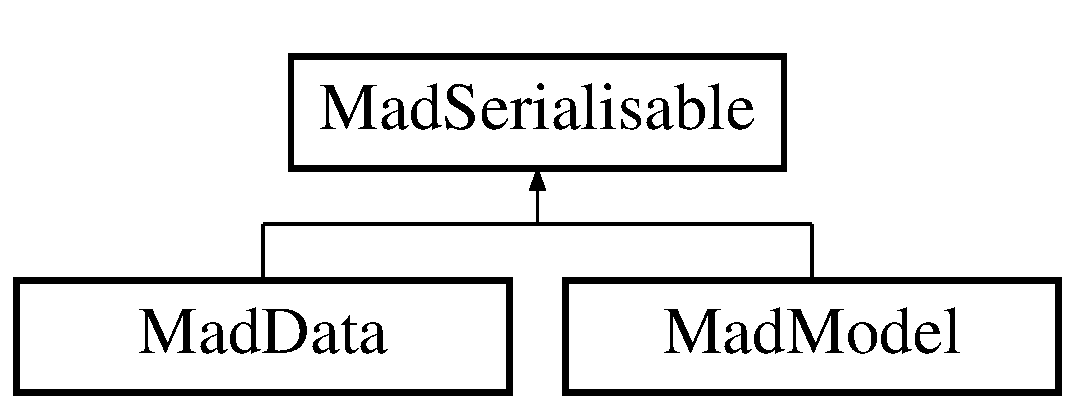
\includegraphics[height=2.000000cm]{class_mad_serialisable}
\end{center}
\end{figure}
\subsection*{Public Member Functions}
\begin{DoxyCompactItemize}
\item 
\hyperlink{class_mad_serialisable_aa2f63236e869cf3237cf4b31194550c5}{Mad\-Serialisable} ()
\begin{DoxyCompactList}\small\item\em \hyperlink{class_mad_serialisable}{Mad\-Serialisable} Constructor. \end{DoxyCompactList}\item 
virtual Q\-String \hyperlink{class_mad_serialisable_ad54654484660b5b0391f5e8765070ec8}{to\-Xml} ()=0
\begin{DoxyCompactList}\small\item\em to\-Xml Write this object to xml and return result as qstring (virtual) \end{DoxyCompactList}\item 
virtual bool \hyperlink{class_mad_serialisable_a59ebe72f565f96ca7cae16f4a4f100b8}{to\-Xml\-File} (const Q\-String the\-File\-Name)
\begin{DoxyCompactList}\small\item\em to\-Xml\-File writes object to xml and return result (virtual qstring) We provide a basic default implementation where given a file name, we will write the serialised xml to that file. Internally it uses \hyperlink{class_mad_serialisable_ad54654484660b5b0391f5e8765070ec8}{to\-Xml()} method so that must be properly implemented. \end{DoxyCompactList}\item 
virtual bool \hyperlink{class_mad_serialisable_a37d5fc3b08cddd05c4ddffdf3fd43535}{from\-Xml} (const Q\-String the\-Xml)=0
\begin{DoxyCompactList}\small\item\em from\-Xml Read this object from xml \end{DoxyCompactList}\item 
virtual bool \hyperlink{class_mad_serialisable_a132a3ea21578307ae1afe074acc20d47}{from\-Xml\-File} (const Q\-String the\-File\-Name)
\begin{DoxyCompactList}\small\item\em from\-Xml\-File Read this object from xml in a file \end{DoxyCompactList}\end{DoxyCompactItemize}


\subsection{Detailed Description}
An abstract base class for any class that is serialiseable to xml \begin{DoxyAuthor}{Author}
Tim Sutton, Jason Jorgenson 
\end{DoxyAuthor}


Definition at line 50 of file madserialisable.\-h.



\subsection{Constructor \& Destructor Documentation}
\hypertarget{class_mad_serialisable_aa2f63236e869cf3237cf4b31194550c5}{\index{Mad\-Serialisable@{Mad\-Serialisable}!Mad\-Serialisable@{Mad\-Serialisable}}
\index{Mad\-Serialisable@{Mad\-Serialisable}!MadSerialisable@{Mad\-Serialisable}}
\subsubsection[{Mad\-Serialisable}]{\setlength{\rightskip}{0pt plus 5cm}Mad\-Serialisable\-::\-Mad\-Serialisable (
\begin{DoxyParamCaption}
{}
\end{DoxyParamCaption}
)}}\label{class_mad_serialisable_aa2f63236e869cf3237cf4b31194550c5}


\hyperlink{class_mad_serialisable}{Mad\-Serialisable} Constructor. 



Definition at line 49 of file madserialisable.\-cpp.



\subsection{Member Function Documentation}
\hypertarget{class_mad_serialisable_a37d5fc3b08cddd05c4ddffdf3fd43535}{\index{Mad\-Serialisable@{Mad\-Serialisable}!from\-Xml@{from\-Xml}}
\index{from\-Xml@{from\-Xml}!MadSerialisable@{Mad\-Serialisable}}
\subsubsection[{from\-Xml}]{\setlength{\rightskip}{0pt plus 5cm}virtual bool Mad\-Serialisable\-::from\-Xml (
\begin{DoxyParamCaption}
\item[{const Q\-String}]{the\-Xml}
\end{DoxyParamCaption}
)\hspace{0.3cm}{\ttfamily [pure virtual]}}}\label{class_mad_serialisable_a37d5fc3b08cddd05c4ddffdf3fd43535}


from\-Xml Read this object from xml 


\begin{DoxyParams}{Parameters}
{\em the\-Xml} & \\
\hline
\end{DoxyParams}
\begin{DoxyReturn}{Returns}
result as true for success, false for failure (virtual) 
\end{DoxyReturn}


Implemented in \hyperlink{class_mad_data_a30677cb8685255a7939d401121525fb6}{Mad\-Data}, and \hyperlink{class_mad_model_ada33c0eed39499b58d0a886566732607}{Mad\-Model}.

\hypertarget{class_mad_serialisable_a132a3ea21578307ae1afe074acc20d47}{\index{Mad\-Serialisable@{Mad\-Serialisable}!from\-Xml\-File@{from\-Xml\-File}}
\index{from\-Xml\-File@{from\-Xml\-File}!MadSerialisable@{Mad\-Serialisable}}
\subsubsection[{from\-Xml\-File}]{\setlength{\rightskip}{0pt plus 5cm}bool Mad\-Serialisable\-::from\-Xml\-File (
\begin{DoxyParamCaption}
\item[{const Q\-String}]{the\-File\-Name}
\end{DoxyParamCaption}
)\hspace{0.3cm}{\ttfamily [virtual]}}}\label{class_mad_serialisable_a132a3ea21578307ae1afe074acc20d47}


from\-Xml\-File Read this object from xml in a file 

\begin{DoxySeeAlso}{See Also}
\hyperlink{class_mad_serialisable_a132a3ea21578307ae1afe074acc20d47}{from\-Xml\-File()} Internally it uses \hyperlink{class_mad_serialisable_a37d5fc3b08cddd05c4ddffdf3fd43535}{from\-Xml(\-Q\-String)} so that must be properly implemented 
\end{DoxySeeAlso}

\begin{DoxyParams}{Parameters}
{\em the\-File\-Name} & \\
\hline
\end{DoxyParams}
\begin{DoxyReturn}{Returns}
result as true for success, false for failure. 
\end{DoxyReturn}


Definition at line 76 of file madserialisable.\-cpp.

\hypertarget{class_mad_serialisable_ad54654484660b5b0391f5e8765070ec8}{\index{Mad\-Serialisable@{Mad\-Serialisable}!to\-Xml@{to\-Xml}}
\index{to\-Xml@{to\-Xml}!MadSerialisable@{Mad\-Serialisable}}
\subsubsection[{to\-Xml}]{\setlength{\rightskip}{0pt plus 5cm}virtual Q\-String Mad\-Serialisable\-::to\-Xml (
\begin{DoxyParamCaption}
{}
\end{DoxyParamCaption}
)\hspace{0.3cm}{\ttfamily [pure virtual]}}}\label{class_mad_serialisable_ad54654484660b5b0391f5e8765070ec8}


to\-Xml Write this object to xml and return result as qstring (virtual) 

Desctructor . \begin{DoxyReturn}{Returns}

\end{DoxyReturn}


Implemented in \hyperlink{class_mad_data_a73665b8eef0518c8c9b2df7d7565f5f8}{Mad\-Data}, and \hyperlink{class_mad_model_a797ce6bb5f6f2798640ef505ed1ee644}{Mad\-Model}.

\hypertarget{class_mad_serialisable_a59ebe72f565f96ca7cae16f4a4f100b8}{\index{Mad\-Serialisable@{Mad\-Serialisable}!to\-Xml\-File@{to\-Xml\-File}}
\index{to\-Xml\-File@{to\-Xml\-File}!MadSerialisable@{Mad\-Serialisable}}
\subsubsection[{to\-Xml\-File}]{\setlength{\rightskip}{0pt plus 5cm}bool Mad\-Serialisable\-::to\-Xml\-File (
\begin{DoxyParamCaption}
\item[{const Q\-String}]{the\-File\-Name}
\end{DoxyParamCaption}
)\hspace{0.3cm}{\ttfamily [virtual]}}}\label{class_mad_serialisable_a59ebe72f565f96ca7cae16f4a4f100b8}


to\-Xml\-File writes object to xml and return result (virtual qstring) We provide a basic default implementation where given a file name, we will write the serialised xml to that file. Internally it uses \hyperlink{class_mad_serialisable_ad54654484660b5b0391f5e8765070ec8}{to\-Xml()} method so that must be properly implemented. 

\begin{DoxySeeAlso}{See Also}
\hyperlink{class_mad_serialisable_ad54654484660b5b0391f5e8765070ec8}{to\-Xml()} 
\end{DoxySeeAlso}

\begin{DoxyParams}{Parameters}
{\em the\-File\-Name} & \\
\hline
\end{DoxyParams}
\begin{DoxyReturn}{Returns}
Q\-String (virtual) 
\end{DoxyReturn}


Definition at line 57 of file madserialisable.\-cpp.



The documentation for this class was generated from the following files\-:\begin{DoxyCompactItemize}
\item 
/\-Users/arkygeek/\-Qt\-Projects/macsur-\/adapter/src/\-Macsur\-Adapter/lib/\hyperlink{madserialisable_8h}{madserialisable.\-h}\item 
/\-Users/arkygeek/\-Qt\-Projects/macsur-\/adapter/src/\-Macsur\-Adapter/lib/\hyperlink{madserialisable_8cpp}{madserialisable.\-cpp}\end{DoxyCompactItemize}

\hypertarget{struct_mad_sub_category}{\section{Mad\-Sub\-Category Struct Reference}
\label{struct_mad_sub_category}\index{Mad\-Sub\-Category@{Mad\-Sub\-Category}}
}


{\ttfamily \#include $<$maddata.\-h$>$}

\subsection*{Public Attributes}
\begin{DoxyCompactItemize}
\item 
Q\-String \hyperlink{struct_mad_sub_category_a0f0d32eb25cfe2236b5b68a65f3bda0a}{name}
\item 
bool \hyperlink{struct_mad_sub_category_a3728af78f99ce0a8c3be3165626862db}{min\-Data}
\item 
float \hyperlink{struct_mad_sub_category_a5514fc9730d13a3c18eaf002bf96bd72}{depth}
\item 
int \hyperlink{struct_mad_sub_category_a7ac12663efbd43f8bb85449c4783523d}{observations}
\item 
float \hyperlink{struct_mad_sub_category_a5aa8b532f2decce8a584b7cbb2b0816c}{weight\-Points}
\item 
int \hyperlink{struct_mad_sub_category_aa2238ad9a0d06d1d35c88c6c6c508270}{replicates}
\end{DoxyCompactItemize}


\subsection{Detailed Description}


Definition at line 43 of file maddata.\-h.



\subsection{Member Data Documentation}
\hypertarget{struct_mad_sub_category_a5514fc9730d13a3c18eaf002bf96bd72}{\index{Mad\-Sub\-Category@{Mad\-Sub\-Category}!depth@{depth}}
\index{depth@{depth}!MadSubCategory@{Mad\-Sub\-Category}}
\subsubsection[{depth}]{\setlength{\rightskip}{0pt plus 5cm}float Mad\-Sub\-Category\-::depth}}\label{struct_mad_sub_category_a5514fc9730d13a3c18eaf002bf96bd72}


Definition at line 47 of file maddata.\-h.

\hypertarget{struct_mad_sub_category_a3728af78f99ce0a8c3be3165626862db}{\index{Mad\-Sub\-Category@{Mad\-Sub\-Category}!min\-Data@{min\-Data}}
\index{min\-Data@{min\-Data}!MadSubCategory@{Mad\-Sub\-Category}}
\subsubsection[{min\-Data}]{\setlength{\rightskip}{0pt plus 5cm}bool Mad\-Sub\-Category\-::min\-Data}}\label{struct_mad_sub_category_a3728af78f99ce0a8c3be3165626862db}


Definition at line 46 of file maddata.\-h.

\hypertarget{struct_mad_sub_category_a0f0d32eb25cfe2236b5b68a65f3bda0a}{\index{Mad\-Sub\-Category@{Mad\-Sub\-Category}!name@{name}}
\index{name@{name}!MadSubCategory@{Mad\-Sub\-Category}}
\subsubsection[{name}]{\setlength{\rightskip}{0pt plus 5cm}Q\-String Mad\-Sub\-Category\-::name}}\label{struct_mad_sub_category_a0f0d32eb25cfe2236b5b68a65f3bda0a}


Definition at line 45 of file maddata.\-h.

\hypertarget{struct_mad_sub_category_a7ac12663efbd43f8bb85449c4783523d}{\index{Mad\-Sub\-Category@{Mad\-Sub\-Category}!observations@{observations}}
\index{observations@{observations}!MadSubCategory@{Mad\-Sub\-Category}}
\subsubsection[{observations}]{\setlength{\rightskip}{0pt plus 5cm}int Mad\-Sub\-Category\-::observations}}\label{struct_mad_sub_category_a7ac12663efbd43f8bb85449c4783523d}


Definition at line 48 of file maddata.\-h.

\hypertarget{struct_mad_sub_category_aa2238ad9a0d06d1d35c88c6c6c508270}{\index{Mad\-Sub\-Category@{Mad\-Sub\-Category}!replicates@{replicates}}
\index{replicates@{replicates}!MadSubCategory@{Mad\-Sub\-Category}}
\subsubsection[{replicates}]{\setlength{\rightskip}{0pt plus 5cm}int Mad\-Sub\-Category\-::replicates}}\label{struct_mad_sub_category_aa2238ad9a0d06d1d35c88c6c6c508270}


Definition at line 50 of file maddata.\-h.

\hypertarget{struct_mad_sub_category_a5aa8b532f2decce8a584b7cbb2b0816c}{\index{Mad\-Sub\-Category@{Mad\-Sub\-Category}!weight\-Points@{weight\-Points}}
\index{weight\-Points@{weight\-Points}!MadSubCategory@{Mad\-Sub\-Category}}
\subsubsection[{weight\-Points}]{\setlength{\rightskip}{0pt plus 5cm}float Mad\-Sub\-Category\-::weight\-Points}}\label{struct_mad_sub_category_a5aa8b532f2decce8a584b7cbb2b0816c}


Definition at line 49 of file maddata.\-h.



The documentation for this struct was generated from the following file\-:\begin{DoxyCompactItemize}
\item 
/\-Users/arkygeek/\-Qt\-Projects/macsur-\/adapter/src/\-Macsur\-Adapter/lib/\hyperlink{maddata_8h}{maddata.\-h}\end{DoxyCompactItemize}

\hypertarget{class_mad_utils}{\section{Mad\-Utils Class Reference}
\label{class_mad_utils}\index{Mad\-Utils@{Mad\-Utils}}
}


{\ttfamily \#include $<$madutils.\-h$>$}

\subsection*{Public Types}
\begin{DoxyCompactItemize}
\item 
typedef Q\-Map$<$ Q\-String, \hyperlink{class_mad_model}{Mad\-Model} $>$ \hyperlink{class_mad_utils_a6bec5016d103cb2712d7bd2001c55b3b}{Model\-Map}
\begin{DoxyCompactList}\small\item\em Model\-Map (typedef) This typedef is used to refer to a collection of layersets. the key is the layerset name the value is the layerset itself. \end{DoxyCompactList}\end{DoxyCompactItemize}
\subsection*{Public Member Functions}
\begin{DoxyCompactItemize}
\item 
\hyperlink{class_mad_utils_a1a74572145ae5f7f6680896bb8fccb0e}{Mad\-Utils} ()
\item 
Q\-String \hyperlink{class_mad_utils_a5c0a97189ce985a39dcd3f3c6882418f}{open\-Graphic\-File} ()
\item 
Q\-String \hyperlink{class_mad_utils_ab4c61234d51b19693917dd0551ad744c}{save\-File} ()
\end{DoxyCompactItemize}
\subsection*{Static Public Member Functions}
\begin{DoxyCompactItemize}
\item 
static const Q\-String \hyperlink{class_mad_utils_a615810cd3a1f9894731a51c5f9cc3e69}{user\-Settings\-Dir\-Path} ()
\begin{DoxyCompactList}\small\item\em user\-Settings\-Dir\-Path Find the place on the filesystem where user data is stored \end{DoxyCompactList}\item 
static const Q\-String \hyperlink{class_mad_utils_aeaed9eea3735e2fa84059b1cd73c9bdd}{user\-Model\-Profiles\-Dir\-Path} ()
\begin{DoxyCompactList}\small\item\em uer\-Model\-Profiles\-Dir\-Path Find the place on the filesystem where user defined model profiles are stored. \end{DoxyCompactList}\item 
static const Q\-String \hyperlink{class_mad_utils_ac79920c4e62df9e73cdc7f5c7675d93f}{user\-Model\-Parameters\-Dir\-Path} ()
\begin{DoxyCompactList}\small\item\em user\-Model\-Parameters\-Dir\-Path Find the place on the filesystem where user defined model parameter profiles are stored. \end{DoxyCompactList}\item 
static const Q\-String \hyperlink{class_mad_utils_a027a1b9a97c1eb82539af3ea971ca73f}{get\-Model\-Output\-Dir} ()
\begin{DoxyCompactList}\small\item\em get\-Model\-Output\-Dir Get the place where model outputs are to be stored. By default this is in $\sim$/.macsur\-Adapter/model\-Outputs But if model\-Outputs\-Dir is specified in Q\-Settings, it will override the default. \end{DoxyCompactList}\item 
static const Q\-String \hyperlink{class_mad_utils_a76f1053d29df630d965a41830920257a}{user\-Images\-Dir\-Path} ()
\begin{DoxyCompactList}\small\item\em user\-Images\-Dir\-Path Find the place on the filesystem where user images are stored. \end{DoxyCompactList}\item 
static \hyperlink{class_mad_utils_a6bec5016d103cb2712d7bd2001c55b3b}{Mad\-Utils\-::\-Model\-Map} \hyperlink{class_mad_utils_ac4ada50d41fccd2f0782c669721165c6}{get\-Available\-Models} ()
\begin{DoxyCompactList}\small\item\em get\-Available\-Models Get a Q\-Map of the avaliable layersets in the users layersets directory \end{DoxyCompactList}\item 
static \hyperlink{class_mad_model}{Mad\-Model} \hyperlink{class_mad_utils_a25b56990e934963c77f010382c92747c}{get\-Model} (Q\-String the\-Guid)
\begin{DoxyCompactList}\small\item\em get\-Model Get a \hyperlink{class_mad_model}{Mad\-Model} given its G\-U\-I\-D. If no matching model is found, a blank one is returned. \end{DoxyCompactList}\item 
static Q\-String\-List \hyperlink{class_mad_utils_a7b39b00a2403f195eee4fc4e510db90b}{sort\-List} (Q\-String\-List the\-List)
\begin{DoxyCompactList}\small\item\em sort\-List Sort a string list into descending alphabetic order and return the result. \end{DoxyCompactList}\item 
static Q\-String\-List \hyperlink{class_mad_utils_a95cfacb1aabb5fd8085933ee9cabb5de}{unique\-List} (Q\-String\-List the\-List)
\begin{DoxyCompactList}\small\item\em unique\-List Remove any duplucate entries from a sorted list \end{DoxyCompactList}\item 
static bool \hyperlink{class_mad_utils_a548aac989563c538ad9695e10845e3ab}{create\-Text\-File} (Q\-String the\-File\-Name, Q\-String the\-Data)
\begin{DoxyCompactList}\small\item\em create\-Text\-File A helper method to easily write a file to disk. \end{DoxyCompactList}\item 
static Q\-String \hyperlink{class_mad_utils_ae6d98beebaf217ce2d630644412eabf2}{xml\-Encode} (Q\-String the\-String)
\begin{DoxyCompactList}\small\item\em xml\-Encode A helper method to xml encode any special chars in a string ($<$ $>$ \& etc) will become ($<$ $>$ \& etc) \end{DoxyCompactList}\item 
static Q\-String \hyperlink{class_mad_utils_aee37612e0cc8aeafe2614b018e5d2c4d}{xml\-Decode} (Q\-String the\-String)
\begin{DoxyCompactList}\small\item\em xml\-Decode A helper method to xml deencode any special chars in a string ($<$ $>$ \& etc) will become ($<$ $>$ \& etc) \end{DoxyCompactList}\item 
static Q\-String \hyperlink{class_mad_utils_ac633dc293b02664fe0246be01a3f448c}{get\-Standard\-Css} ()
\begin{DoxyCompactList}\small\item\em get\-Standard\-Css Get the standard style sheet for reports. Typically this will be used like this\-: Q\-String my\-Style = \hyperlink{class_mad_utils_ac633dc293b02664fe0246be01a3f448c}{get\-Standard\-Css()}; text\-Browser\-Foo-\/$>$document()-\/$>$set\-Default\-Stylesheet(my\-Style); \end{DoxyCompactList}\item 
static const Q\-String \hyperlink{class_mad_utils_add01d28ed02067656f7f20240c9b8213}{user\-Conversion\-Tables\-Dir\-Path} ()
\end{DoxyCompactItemize}


\subsection{Detailed Description}


Definition at line 41 of file madutils.\-h.



\subsection{Member Typedef Documentation}
\hypertarget{class_mad_utils_a6bec5016d103cb2712d7bd2001c55b3b}{\index{Mad\-Utils@{Mad\-Utils}!Model\-Map@{Model\-Map}}
\index{Model\-Map@{Model\-Map}!MadUtils@{Mad\-Utils}}
\subsubsection[{Model\-Map}]{\setlength{\rightskip}{0pt plus 5cm}typedef Q\-Map$<$Q\-String,{\bf Mad\-Model}$>$ {\bf Mad\-Utils\-::\-Model\-Map}}}\label{class_mad_utils_a6bec5016d103cb2712d7bd2001c55b3b}


Model\-Map (typedef) This typedef is used to refer to a collection of layersets. the key is the layerset name the value is the layerset itself. 



Definition at line 101 of file madutils.\-h.



\subsection{Constructor \& Destructor Documentation}
\hypertarget{class_mad_utils_a1a74572145ae5f7f6680896bb8fccb0e}{\index{Mad\-Utils@{Mad\-Utils}!Mad\-Utils@{Mad\-Utils}}
\index{Mad\-Utils@{Mad\-Utils}!MadUtils@{Mad\-Utils}}
\subsubsection[{Mad\-Utils}]{\setlength{\rightskip}{0pt plus 5cm}Mad\-Utils\-::\-Mad\-Utils (
\begin{DoxyParamCaption}
{}
\end{DoxyParamCaption}
)}}\label{class_mad_utils_a1a74572145ae5f7f6680896bb8fccb0e}


Definition at line 44 of file madutils.\-cpp.



\subsection{Member Function Documentation}
\hypertarget{class_mad_utils_a548aac989563c538ad9695e10845e3ab}{\index{Mad\-Utils@{Mad\-Utils}!create\-Text\-File@{create\-Text\-File}}
\index{create\-Text\-File@{create\-Text\-File}!MadUtils@{Mad\-Utils}}
\subsubsection[{create\-Text\-File}]{\setlength{\rightskip}{0pt plus 5cm}bool Mad\-Utils\-::create\-Text\-File (
\begin{DoxyParamCaption}
\item[{Q\-String}]{the\-File\-Name, }
\item[{Q\-String}]{the\-Data}
\end{DoxyParamCaption}
)\hspace{0.3cm}{\ttfamily [static]}}}\label{class_mad_utils_a548aac989563c538ad9695e10845e3ab}


create\-Text\-File A helper method to easily write a file to disk. 


\begin{DoxyParams}{Parameters}
{\em the\-File\-Name} & -\/ the filename to be created or overwritten \\
\hline
{\em the\-Data} & -\/ the data that will be written into the file \\
\hline
\end{DoxyParams}
\begin{DoxyReturn}{Returns}
bool -\/ false if the file could not be written 
\end{DoxyReturn}


Definition at line 126 of file madutils.\-cpp.

\hypertarget{class_mad_utils_ac4ada50d41fccd2f0782c669721165c6}{\index{Mad\-Utils@{Mad\-Utils}!get\-Available\-Models@{get\-Available\-Models}}
\index{get\-Available\-Models@{get\-Available\-Models}!MadUtils@{Mad\-Utils}}
\subsubsection[{get\-Available\-Models}]{\setlength{\rightskip}{0pt plus 5cm}{\bf Mad\-Utils\-::\-Model\-Map} Mad\-Utils\-::get\-Available\-Models (
\begin{DoxyParamCaption}
{}
\end{DoxyParamCaption}
)\hspace{0.3cm}{\ttfamily [static]}}}\label{class_mad_utils_ac4ada50d41fccd2f0782c669721165c6}


get\-Available\-Models Get a Q\-Map of the avaliable layersets in the users layersets directory 

\begin{DoxyReturn}{Returns}
a Q\-Map$<$\-Q\-String,\-Omg\-Layer\-Set$>$ where the Q\-String key is the layerset name 
\end{DoxyReturn}


Definition at line 93 of file madutils.\-cpp.

\hypertarget{class_mad_utils_a25b56990e934963c77f010382c92747c}{\index{Mad\-Utils@{Mad\-Utils}!get\-Model@{get\-Model}}
\index{get\-Model@{get\-Model}!MadUtils@{Mad\-Utils}}
\subsubsection[{get\-Model}]{\setlength{\rightskip}{0pt plus 5cm}static {\bf Mad\-Model} Mad\-Utils\-::get\-Model (
\begin{DoxyParamCaption}
\item[{Q\-String}]{the\-Guid}
\end{DoxyParamCaption}
)\hspace{0.3cm}{\ttfamily [static]}}}\label{class_mad_utils_a25b56990e934963c77f010382c92747c}


get\-Model Get a \hyperlink{class_mad_model}{Mad\-Model} given its G\-U\-I\-D. If no matching model is found, a blank one is returned. 

\hypertarget{class_mad_utils_a027a1b9a97c1eb82539af3ea971ca73f}{\index{Mad\-Utils@{Mad\-Utils}!get\-Model\-Output\-Dir@{get\-Model\-Output\-Dir}}
\index{get\-Model\-Output\-Dir@{get\-Model\-Output\-Dir}!MadUtils@{Mad\-Utils}}
\subsubsection[{get\-Model\-Output\-Dir}]{\setlength{\rightskip}{0pt plus 5cm}const Q\-String Mad\-Utils\-::get\-Model\-Output\-Dir (
\begin{DoxyParamCaption}
{}
\end{DoxyParamCaption}
)\hspace{0.3cm}{\ttfamily [static]}}}\label{class_mad_utils_a027a1b9a97c1eb82539af3ea971ca73f}


get\-Model\-Output\-Dir Get the place where model outputs are to be stored. By default this is in $\sim$/.macsur\-Adapter/model\-Outputs But if model\-Outputs\-Dir is specified in Q\-Settings, it will override the default. 



Definition at line 60 of file madutils.\-cpp.

\hypertarget{class_mad_utils_ac633dc293b02664fe0246be01a3f448c}{\index{Mad\-Utils@{Mad\-Utils}!get\-Standard\-Css@{get\-Standard\-Css}}
\index{get\-Standard\-Css@{get\-Standard\-Css}!MadUtils@{Mad\-Utils}}
\subsubsection[{get\-Standard\-Css}]{\setlength{\rightskip}{0pt plus 5cm}Q\-String Mad\-Utils\-::get\-Standard\-Css (
\begin{DoxyParamCaption}
{}
\end{DoxyParamCaption}
)\hspace{0.3cm}{\ttfamily [static]}}}\label{class_mad_utils_ac633dc293b02664fe0246be01a3f448c}


get\-Standard\-Css Get the standard style sheet for reports. Typically this will be used like this\-: Q\-String my\-Style = \hyperlink{class_mad_utils_ac633dc293b02664fe0246be01a3f448c}{get\-Standard\-Css()}; text\-Browser\-Foo-\/$>$document()-\/$>$set\-Default\-Stylesheet(my\-Style); 



Definition at line 159 of file madutils.\-cpp.

\hypertarget{class_mad_utils_a5c0a97189ce985a39dcd3f3c6882418f}{\index{Mad\-Utils@{Mad\-Utils}!open\-Graphic\-File@{open\-Graphic\-File}}
\index{open\-Graphic\-File@{open\-Graphic\-File}!MadUtils@{Mad\-Utils}}
\subsubsection[{open\-Graphic\-File}]{\setlength{\rightskip}{0pt plus 5cm}Q\-String Mad\-Utils\-::open\-Graphic\-File (
\begin{DoxyParamCaption}
{}
\end{DoxyParamCaption}
)}}\label{class_mad_utils_a5c0a97189ce985a39dcd3f3c6882418f}


Definition at line 180 of file madutils.\-cpp.

\hypertarget{class_mad_utils_ab4c61234d51b19693917dd0551ad744c}{\index{Mad\-Utils@{Mad\-Utils}!save\-File@{save\-File}}
\index{save\-File@{save\-File}!MadUtils@{Mad\-Utils}}
\subsubsection[{save\-File}]{\setlength{\rightskip}{0pt plus 5cm}Q\-String Mad\-Utils\-::save\-File (
\begin{DoxyParamCaption}
{}
\end{DoxyParamCaption}
)}}\label{class_mad_utils_ab4c61234d51b19693917dd0551ad744c}


Definition at line 191 of file madutils.\-cpp.

\hypertarget{class_mad_utils_a7b39b00a2403f195eee4fc4e510db90b}{\index{Mad\-Utils@{Mad\-Utils}!sort\-List@{sort\-List}}
\index{sort\-List@{sort\-List}!MadUtils@{Mad\-Utils}}
\subsubsection[{sort\-List}]{\setlength{\rightskip}{0pt plus 5cm}static Q\-String\-List Mad\-Utils\-::sort\-List (
\begin{DoxyParamCaption}
\item[{Q\-String\-List}]{the\-List}
\end{DoxyParamCaption}
)\hspace{0.3cm}{\ttfamily [static]}}}\label{class_mad_utils_a7b39b00a2403f195eee4fc4e510db90b}


sort\-List Sort a string list into descending alphabetic order and return the result. 


\begin{DoxyParams}{Parameters}
{\em the\-List} & -\/ the Q\-String\-List to be sorted \\
\hline
\end{DoxyParams}
\begin{DoxyReturn}{Returns}
Q\-String\-List -\/ sorted in descending alphabetical order 
\end{DoxyReturn}
\hypertarget{class_mad_utils_a95cfacb1aabb5fd8085933ee9cabb5de}{\index{Mad\-Utils@{Mad\-Utils}!unique\-List@{unique\-List}}
\index{unique\-List@{unique\-List}!MadUtils@{Mad\-Utils}}
\subsubsection[{unique\-List}]{\setlength{\rightskip}{0pt plus 5cm}static Q\-String\-List Mad\-Utils\-::unique\-List (
\begin{DoxyParamCaption}
\item[{Q\-String\-List}]{the\-List}
\end{DoxyParamCaption}
)\hspace{0.3cm}{\ttfamily [static]}}}\label{class_mad_utils_a95cfacb1aabb5fd8085933ee9cabb5de}


unique\-List Remove any duplucate entries from a sorted list 


\begin{DoxyParams}{Parameters}
{\em the\-List} & -\/ the Q\-String\-List to be sorted \\
\hline
\end{DoxyParams}
\begin{DoxyReturn}{Returns}
Q\-String\-List -\/ a list with no sequential duplicates 
\end{DoxyReturn}
\hypertarget{class_mad_utils_add01d28ed02067656f7f20240c9b8213}{\index{Mad\-Utils@{Mad\-Utils}!user\-Conversion\-Tables\-Dir\-Path@{user\-Conversion\-Tables\-Dir\-Path}}
\index{user\-Conversion\-Tables\-Dir\-Path@{user\-Conversion\-Tables\-Dir\-Path}!MadUtils@{Mad\-Utils}}
\subsubsection[{user\-Conversion\-Tables\-Dir\-Path}]{\setlength{\rightskip}{0pt plus 5cm}const Q\-String Mad\-Utils\-::user\-Conversion\-Tables\-Dir\-Path (
\begin{DoxyParamCaption}
{}
\end{DoxyParamCaption}
)\hspace{0.3cm}{\ttfamily [static]}}}\label{class_mad_utils_add01d28ed02067656f7f20240c9b8213}
Find the place on the filesystem where user created conversion tables in csv format are stored

Typically this will be $\sim$/.macsur\-Adapter/conversion\-Tables

\begin{DoxyReturn}{Returns}
Q\-String containing the relevant directory name 
\end{DoxyReturn}


Definition at line 201 of file madutils.\-cpp.

\hypertarget{class_mad_utils_a76f1053d29df630d965a41830920257a}{\index{Mad\-Utils@{Mad\-Utils}!user\-Images\-Dir\-Path@{user\-Images\-Dir\-Path}}
\index{user\-Images\-Dir\-Path@{user\-Images\-Dir\-Path}!MadUtils@{Mad\-Utils}}
\subsubsection[{user\-Images\-Dir\-Path}]{\setlength{\rightskip}{0pt plus 5cm}const Q\-String Mad\-Utils\-::user\-Images\-Dir\-Path (
\begin{DoxyParamCaption}
{}
\end{DoxyParamCaption}
)\hspace{0.3cm}{\ttfamily [static]}}}\label{class_mad_utils_a76f1053d29df630d965a41830920257a}


user\-Images\-Dir\-Path Find the place on the filesystem where user images are stored. 

Typically this will be $\sim$/.macsur\-Adapter/images

\begin{DoxyReturn}{Returns}
Q\-String containing the relevant directory name 
\end{DoxyReturn}


Definition at line 85 of file madutils.\-cpp.

\hypertarget{class_mad_utils_ac79920c4e62df9e73cdc7f5c7675d93f}{\index{Mad\-Utils@{Mad\-Utils}!user\-Model\-Parameters\-Dir\-Path@{user\-Model\-Parameters\-Dir\-Path}}
\index{user\-Model\-Parameters\-Dir\-Path@{user\-Model\-Parameters\-Dir\-Path}!MadUtils@{Mad\-Utils}}
\subsubsection[{user\-Model\-Parameters\-Dir\-Path}]{\setlength{\rightskip}{0pt plus 5cm}const Q\-String Mad\-Utils\-::user\-Model\-Parameters\-Dir\-Path (
\begin{DoxyParamCaption}
{}
\end{DoxyParamCaption}
)\hspace{0.3cm}{\ttfamily [static]}}}\label{class_mad_utils_ac79920c4e62df9e73cdc7f5c7675d93f}


user\-Model\-Parameters\-Dir\-Path Find the place on the filesystem where user defined model parameter profiles are stored. 

Typically this will be $\sim$/.macsur\-Adapter/animal\-Parameters

\begin{DoxyReturn}{Returns}
Q\-String containing the relevant directory name 
\end{DoxyReturn}


Definition at line 76 of file madutils.\-cpp.

\hypertarget{class_mad_utils_aeaed9eea3735e2fa84059b1cd73c9bdd}{\index{Mad\-Utils@{Mad\-Utils}!user\-Model\-Profiles\-Dir\-Path@{user\-Model\-Profiles\-Dir\-Path}}
\index{user\-Model\-Profiles\-Dir\-Path@{user\-Model\-Profiles\-Dir\-Path}!MadUtils@{Mad\-Utils}}
\subsubsection[{user\-Model\-Profiles\-Dir\-Path}]{\setlength{\rightskip}{0pt plus 5cm}const Q\-String Mad\-Utils\-::user\-Model\-Profiles\-Dir\-Path (
\begin{DoxyParamCaption}
{}
\end{DoxyParamCaption}
)\hspace{0.3cm}{\ttfamily [static]}}}\label{class_mad_utils_aeaed9eea3735e2fa84059b1cd73c9bdd}


uer\-Model\-Profiles\-Dir\-Path Find the place on the filesystem where user defined model profiles are stored. 

Typically this will be $\sim$/.macsur\-Adapter/model\-Profiles

\begin{DoxyReturn}{Returns}
Q\-String containing the relevant directory name 
\end{DoxyReturn}


Definition at line 67 of file madutils.\-cpp.

\hypertarget{class_mad_utils_a615810cd3a1f9894731a51c5f9cc3e69}{\index{Mad\-Utils@{Mad\-Utils}!user\-Settings\-Dir\-Path@{user\-Settings\-Dir\-Path}}
\index{user\-Settings\-Dir\-Path@{user\-Settings\-Dir\-Path}!MadUtils@{Mad\-Utils}}
\subsubsection[{user\-Settings\-Dir\-Path}]{\setlength{\rightskip}{0pt plus 5cm}const Q\-String Mad\-Utils\-::user\-Settings\-Dir\-Path (
\begin{DoxyParamCaption}
{}
\end{DoxyParamCaption}
)\hspace{0.3cm}{\ttfamily [static]}}}\label{class_mad_utils_a615810cd3a1f9894731a51c5f9cc3e69}


user\-Settings\-Dir\-Path Find the place on the filesystem where user data is stored 

Typically, this will be $\sim$/.macsur\-Adapter

\begin{DoxyReturn}{Returns}
Q\-String containing the relevant directory name
\end{DoxyReturn}
Returns the path to the settings directory in user's home dir 

Definition at line 51 of file madutils.\-cpp.

\hypertarget{class_mad_utils_aee37612e0cc8aeafe2614b018e5d2c4d}{\index{Mad\-Utils@{Mad\-Utils}!xml\-Decode@{xml\-Decode}}
\index{xml\-Decode@{xml\-Decode}!MadUtils@{Mad\-Utils}}
\subsubsection[{xml\-Decode}]{\setlength{\rightskip}{0pt plus 5cm}Q\-String Mad\-Utils\-::xml\-Decode (
\begin{DoxyParamCaption}
\item[{Q\-String}]{the\-String}
\end{DoxyParamCaption}
)\hspace{0.3cm}{\ttfamily [static]}}}\label{class_mad_utils_aee37612e0cc8aeafe2614b018e5d2c4d}


xml\-Decode A helper method to xml deencode any special chars in a string ($<$ $>$ \& etc) will become ($<$ $>$ \& etc) 


\begin{DoxyParams}{Parameters}
{\em Q\-String} & -\/ the string to be properly decoded \\
\hline
\end{DoxyParams}
\begin{DoxyReturn}{Returns}
A Q\-String with the encoded chars properly decoded 
\end{DoxyReturn}


Definition at line 151 of file madutils.\-cpp.

\hypertarget{class_mad_utils_ae6d98beebaf217ce2d630644412eabf2}{\index{Mad\-Utils@{Mad\-Utils}!xml\-Encode@{xml\-Encode}}
\index{xml\-Encode@{xml\-Encode}!MadUtils@{Mad\-Utils}}
\subsubsection[{xml\-Encode}]{\setlength{\rightskip}{0pt plus 5cm}Q\-String Mad\-Utils\-::xml\-Encode (
\begin{DoxyParamCaption}
\item[{Q\-String}]{the\-String}
\end{DoxyParamCaption}
)\hspace{0.3cm}{\ttfamily [static]}}}\label{class_mad_utils_ae6d98beebaf217ce2d630644412eabf2}


xml\-Encode A helper method to xml encode any special chars in a string ($<$ $>$ \& etc) will become ($<$ $>$ \& etc) 


\begin{DoxyParams}{Parameters}
{\em Q\-String} & -\/ the string to be properly encoded \\
\hline
\end{DoxyParams}
\begin{DoxyReturn}{Returns}
A Q\-String with the special chars properly encoded 
\end{DoxyReturn}


Definition at line 143 of file madutils.\-cpp.



The documentation for this class was generated from the following files\-:\begin{DoxyCompactItemize}
\item 
/\-Users/arkygeek/\-Qt\-Projects/macsur-\/adapter/src/\-Macsur\-Adapter/lib/\hyperlink{madutils_8h}{madutils.\-h}\item 
/\-Users/arkygeek/\-Qt\-Projects/macsur-\/adapter/src/\-Macsur\-Adapter/lib/\hyperlink{madutils_8cpp}{madutils.\-cpp}\end{DoxyCompactItemize}

\chapter{File Documentation}
\hypertarget{maddataclassification_8cpp}{\section{/\-Users/arkygeek/\-Qt\-Projects/macsur-\/adapter/src/\-Macsur\-Adapter/gui/maddataclassification.cpp File Reference}
\label{maddataclassification_8cpp}\index{/\-Users/arkygeek/\-Qt\-Projects/macsur-\/adapter/src/\-Macsur\-Adapter/gui/maddataclassification.\-cpp@{/\-Users/arkygeek/\-Qt\-Projects/macsur-\/adapter/src/\-Macsur\-Adapter/gui/maddataclassification.\-cpp}}
}
{\ttfamily \#include $<$iomanip$>$}\\*
{\ttfamily \#include \char`\"{}maddataclassification.\-h\char`\"{}}\\*
{\ttfamily \#include \char`\"{}lib/mad.\-h\char`\"{}}\\*

\hypertarget{maddataclassification_8h}{\section{/\-Users/arkygeek/\-Qt\-Projects/macsur-\/adapter/src/\-Macsur\-Adapter/gui/maddataclassification.h File Reference}
\label{maddataclassification_8h}\index{/\-Users/arkygeek/\-Qt\-Projects/macsur-\/adapter/src/\-Macsur\-Adapter/gui/maddataclassification.\-h@{/\-Users/arkygeek/\-Qt\-Projects/macsur-\/adapter/src/\-Macsur\-Adapter/gui/maddataclassification.\-h}}
}
{\ttfamily \#include \char`\"{}ui\-\_\-maddataclassificationbase.\-h\char`\"{}}\\*
\subsection*{Classes}
\begin{DoxyCompactItemize}
\item 
class \hyperlink{class_mad_data_classification}{Mad\-Data\-Classification}
\end{DoxyCompactItemize}

\hypertarget{mad_8h}{\section{/\-Users/arkygeek/\-Qt\-Projects/macsur-\/adapter/src/\-Macsur\-Adapter/lib/mad.h File Reference}
\label{mad_8h}\index{/\-Users/arkygeek/\-Qt\-Projects/macsur-\/adapter/src/\-Macsur\-Adapter/lib/mad.\-h@{/\-Users/arkygeek/\-Qt\-Projects/macsur-\/adapter/src/\-Macsur\-Adapter/lib/mad.\-h}}
}
{\ttfamily \#include $<$Q\-Map$>$}\\*
{\ttfamily \#include $<$Q\-Pair$>$}\\*
{\ttfamily \#include $<$Q\-String$>$}\\*
{\ttfamily \#include \char`\"{}madmodel.\-h\char`\"{}}\\*
{\ttfamily \#include \char`\"{}maddata.\-h\char`\"{}}\\*
\subsection*{Typedefs}
\begin{DoxyCompactItemize}
\item 
typedef Q\-Map$<$ Q\-String, Q\-Pair\\*
$<$ bool, Q\-String $>$ $>$ \hyperlink{mad_8h_a65e2842c1a6c5851fb16f76cd674ba3e}{Mad\-Triple\-Map}
\begin{DoxyCompactList}\small\item\em Mad\-Triple\-Map. \end{DoxyCompactList}\item 
typedef Q\-Pair$<$ Q\-Pair$<$ Q\-String, \\*
Q\-String $>$, Q\-Pair$<$ Q\-String, \\*
Q\-String $>$ $>$ \hyperlink{mad_8h_ab8f6560b33c97bc52ea007d5ffc6e779}{Mad\-Model\-Info}
\begin{DoxyCompactList}\small\item\em Mad\-Model\-Info. \end{DoxyCompactList}\end{DoxyCompactItemize}
\subsection*{Enumerations}
\begin{DoxyCompactItemize}
\item 
enum \hyperlink{mad_8h_a96ac0e0bcd681699758501ffc8feaaeb}{Model\-Theme} \{ \hyperlink{mad_8h_a96ac0e0bcd681699758501ffc8feaaebad1d7db3049beeda2204cb4660bb8dd82}{Crop\-M}, 
\hyperlink{mad_8h_a96ac0e0bcd681699758501ffc8feaaebaeeb7e832c90579e1cdc6e5a2b80fecf7}{Live\-M}, 
\hyperlink{mad_8h_a96ac0e0bcd681699758501ffc8feaaeba2d61de4025929dd9cbd0084d9b778247}{Trade\-M}
 \}
\begin{DoxyCompactList}\small\item\em Mad\-Model\-Map. \end{DoxyCompactList}\item 
enum \hyperlink{mad_8h_a8e8d3da3ac3510ba6f5aa1a4c8c82eae}{Scale} \{ \\*
\hyperlink{mad_8h_a8e8d3da3ac3510ba6f5aa1a4c8c82eaea12c94ce092e49570747864f9d8fa72d0}{Farm}, 
\hyperlink{mad_8h_a8e8d3da3ac3510ba6f5aa1a4c8c82eaea60584a5fa3c118f79220d9220d26f141}{Locality}, 
\hyperlink{mad_8h_a8e8d3da3ac3510ba6f5aa1a4c8c82eaea023bdd1bf971f4038cba7eb662ea8121}{Region}, 
\hyperlink{mad_8h_a8e8d3da3ac3510ba6f5aa1a4c8c82eaea098929f2e407440bd2b76a53ebba5ed8}{National}, 
\\*
\hyperlink{mad_8h_a8e8d3da3ac3510ba6f5aa1a4c8c82eaea26d4759cf0159a6e2befbd05f43971cb}{International}, 
\hyperlink{mad_8h_a8e8d3da3ac3510ba6f5aa1a4c8c82eaea03ddcda8467f404189c984dc13409aa8}{Global}
 \}
\begin{DoxyCompactList}\small\item\em The Scale enum. \end{DoxyCompactList}\item 
enum \hyperlink{mad_8h_a5096484b74a71affe0e9f6bd5c079b07}{Nuts} \{ \hyperlink{mad_8h_a5096484b74a71affe0e9f6bd5c079b07adc04b1fc7bbda016eb745bea75642823}{Nuts1}, 
\hyperlink{mad_8h_a5096484b74a71affe0e9f6bd5c079b07a17e985ecd09606f112f182be89ff4ffe}{Nuts2}, 
\hyperlink{mad_8h_a5096484b74a71affe0e9f6bd5c079b07aa28d3371785791caf1a39378a19cc3d9}{Nuts3}
 \}
\begin{DoxyCompactList}\small\item\em The Nuts enum. \end{DoxyCompactList}\item 
enum \hyperlink{mad_8h_ad5c8cac9c62ffdb8a2223362226dee47}{Area\-Units} \{ \\*
\hyperlink{mad_8h_ad5c8cac9c62ffdb8a2223362226dee47a10d869fda8ef9b3852491ed49722a677}{Dunum}, 
\hyperlink{mad_8h_ad5c8cac9c62ffdb8a2223362226dee47a6bf9786325e8633eb9e90667c85b339d}{Hectare}, 
\hyperlink{mad_8h_ad5c8cac9c62ffdb8a2223362226dee47a7c11704f43073bbb124071d1a11a92c0}{Acre}, 
\hyperlink{mad_8h_ad5c8cac9c62ffdb8a2223362226dee47ae166cd5dada4579624e167c4d2771e80}{Square\-Km}, 
\\*
\hyperlink{mad_8h_ad5c8cac9c62ffdb8a2223362226dee47ac15d0645187d53b1cb534224644495b6}{Square\-Mile}
 \}
\begin{DoxyCompactList}\small\item\em The Area\-Units enum. \end{DoxyCompactList}\item 
enum \hyperlink{mad_8h_a2c794c5c13ab4dd7e65bad031dbe41c3}{File\-Type} \{ \hyperlink{mad_8h_a2c794c5c13ab4dd7e65bad031dbe41c3a2b10dde645e767164fc3de2ddbf14399}{C\-S\-V}, 
\hyperlink{mad_8h_a2c794c5c13ab4dd7e65bad031dbe41c3a920380215591395ea33ee5df8e293e19}{T\-A\-B}, 
\hyperlink{mad_8h_a2c794c5c13ab4dd7e65bad031dbe41c3a8b753feec7368928510c5dcd8ad8f7d4}{Other\-Delimited}, 
\hyperlink{mad_8h_a2c794c5c13ab4dd7e65bad031dbe41c3ae27b0860dfa490c46dd387b06d21a04b}{Binary}
 \}
\begin{DoxyCompactList}\small\item\em The File\-Type enum. \end{DoxyCompactList}\item 
enum \hyperlink{mad_8h_a7a6534a55fc72bbcb547056b9eb694ed}{Energy\-Type} \{ \hyperlink{mad_8h_a7a6534a55fc72bbcb547056b9eb694edaf01989f7865a5d3e380a68985117766a}{K\-Calories}, 
\hyperlink{mad_8h_a7a6534a55fc72bbcb547056b9eb694eda1756e3a2172131326e9b700da5cce029}{T\-D\-N}
 \}
\begin{DoxyCompactList}\small\item\em The Energy\-Type enum. \end{DoxyCompactList}\item 
enum \hyperlink{mad_8h_ab6ad47405d01eb611996d855bef0610d}{Data\-Class} \{ \hyperlink{mad_8h_ab6ad47405d01eb611996d855bef0610daba976230e236daa04305650837dfed81}{Platinum}, 
\hyperlink{mad_8h_ab6ad47405d01eb611996d855bef0610da4fe767077a795c957f76faf02f3ca765}{Gold}, 
\hyperlink{mad_8h_ab6ad47405d01eb611996d855bef0610dae7df9b76b384066c07fc2b24fb693fdf}{Silver}, 
\hyperlink{mad_8h_ab6ad47405d01eb611996d855bef0610da251f89ea3c50795a6f8d4f9969df76ea}{Bronze}
 \}
\begin{DoxyCompactList}\small\item\em The Data\-Class enum. \end{DoxyCompactList}\end{DoxyCompactItemize}


\subsection{Typedef Documentation}
\hypertarget{mad_8h_ab8f6560b33c97bc52ea007d5ffc6e779}{\index{mad.\-h@{mad.\-h}!Mad\-Model\-Info@{Mad\-Model\-Info}}
\index{Mad\-Model\-Info@{Mad\-Model\-Info}!mad.h@{mad.\-h}}
\subsubsection[{Mad\-Model\-Info}]{\setlength{\rightskip}{0pt plus 5cm}typedef Q\-Pair$<$Q\-Pair$<$Q\-String,Q\-String$>$, Q\-Pair$<$Q\-String,Q\-String$>$ $>$ {\bf Mad\-Model\-Info}}}\label{mad_8h_ab8f6560b33c97bc52ea007d5ffc6e779}


Mad\-Model\-Info. 



Definition at line 57 of file mad.\-h.

\hypertarget{mad_8h_a65e2842c1a6c5851fb16f76cd674ba3e}{\index{mad.\-h@{mad.\-h}!Mad\-Triple\-Map@{Mad\-Triple\-Map}}
\index{Mad\-Triple\-Map@{Mad\-Triple\-Map}!mad.h@{mad.\-h}}
\subsubsection[{Mad\-Triple\-Map}]{\setlength{\rightskip}{0pt plus 5cm}typedef Q\-Map$<$Q\-String,Q\-Pair$<$bool,Q\-String$>$ $>$ {\bf Mad\-Triple\-Map}}}\label{mad_8h_a65e2842c1a6c5851fb16f76cd674ba3e}


Mad\-Triple\-Map. 



Definition at line 53 of file mad.\-h.



\subsection{Enumeration Type Documentation}
\hypertarget{mad_8h_ad5c8cac9c62ffdb8a2223362226dee47}{\index{mad.\-h@{mad.\-h}!Area\-Units@{Area\-Units}}
\index{Area\-Units@{Area\-Units}!mad.h@{mad.\-h}}
\subsubsection[{Area\-Units}]{\setlength{\rightskip}{0pt plus 5cm}enum {\bf Area\-Units}}}\label{mad_8h_ad5c8cac9c62ffdb8a2223362226dee47}


The Area\-Units enum. 

\begin{Desc}
\item[Enumerator]\par
\begin{description}
\index{Dunum@{Dunum}!mad.\-h@{mad.\-h}}\index{mad.\-h@{mad.\-h}!Dunum@{Dunum}}\item[{\em 
\hypertarget{mad_8h_ad5c8cac9c62ffdb8a2223362226dee47a10d869fda8ef9b3852491ed49722a677}{Dunum}\label{mad_8h_ad5c8cac9c62ffdb8a2223362226dee47a10d869fda8ef9b3852491ed49722a677}
}]\index{Hectare@{Hectare}!mad.\-h@{mad.\-h}}\index{mad.\-h@{mad.\-h}!Hectare@{Hectare}}\item[{\em 
\hypertarget{mad_8h_ad5c8cac9c62ffdb8a2223362226dee47a6bf9786325e8633eb9e90667c85b339d}{Hectare}\label{mad_8h_ad5c8cac9c62ffdb8a2223362226dee47a6bf9786325e8633eb9e90667c85b339d}
}]\index{Acre@{Acre}!mad.\-h@{mad.\-h}}\index{mad.\-h@{mad.\-h}!Acre@{Acre}}\item[{\em 
\hypertarget{mad_8h_ad5c8cac9c62ffdb8a2223362226dee47a7c11704f43073bbb124071d1a11a92c0}{Acre}\label{mad_8h_ad5c8cac9c62ffdb8a2223362226dee47a7c11704f43073bbb124071d1a11a92c0}
}]\index{Square\-Km@{Square\-Km}!mad.\-h@{mad.\-h}}\index{mad.\-h@{mad.\-h}!Square\-Km@{Square\-Km}}\item[{\em 
\hypertarget{mad_8h_ad5c8cac9c62ffdb8a2223362226dee47ae166cd5dada4579624e167c4d2771e80}{Square\-Km}\label{mad_8h_ad5c8cac9c62ffdb8a2223362226dee47ae166cd5dada4579624e167c4d2771e80}
}]\index{Square\-Mile@{Square\-Mile}!mad.\-h@{mad.\-h}}\index{mad.\-h@{mad.\-h}!Square\-Mile@{Square\-Mile}}\item[{\em 
\hypertarget{mad_8h_ad5c8cac9c62ffdb8a2223362226dee47ac15d0645187d53b1cb534224644495b6}{Square\-Mile}\label{mad_8h_ad5c8cac9c62ffdb8a2223362226dee47ac15d0645187d53b1cb534224644495b6}
}]\end{description}
\end{Desc}


Definition at line 78 of file mad.\-h.

\hypertarget{mad_8h_ab6ad47405d01eb611996d855bef0610d}{\index{mad.\-h@{mad.\-h}!Data\-Class@{Data\-Class}}
\index{Data\-Class@{Data\-Class}!mad.h@{mad.\-h}}
\subsubsection[{Data\-Class}]{\setlength{\rightskip}{0pt plus 5cm}enum {\bf Data\-Class}}}\label{mad_8h_ab6ad47405d01eb611996d855bef0610d}


The Data\-Class enum. 

\begin{Desc}
\item[Enumerator]\par
\begin{description}
\index{Platinum@{Platinum}!mad.\-h@{mad.\-h}}\index{mad.\-h@{mad.\-h}!Platinum@{Platinum}}\item[{\em 
\hypertarget{mad_8h_ab6ad47405d01eb611996d855bef0610daba976230e236daa04305650837dfed81}{Platinum}\label{mad_8h_ab6ad47405d01eb611996d855bef0610daba976230e236daa04305650837dfed81}
}]\index{Gold@{Gold}!mad.\-h@{mad.\-h}}\index{mad.\-h@{mad.\-h}!Gold@{Gold}}\item[{\em 
\hypertarget{mad_8h_ab6ad47405d01eb611996d855bef0610da4fe767077a795c957f76faf02f3ca765}{Gold}\label{mad_8h_ab6ad47405d01eb611996d855bef0610da4fe767077a795c957f76faf02f3ca765}
}]\index{Silver@{Silver}!mad.\-h@{mad.\-h}}\index{mad.\-h@{mad.\-h}!Silver@{Silver}}\item[{\em 
\hypertarget{mad_8h_ab6ad47405d01eb611996d855bef0610dae7df9b76b384066c07fc2b24fb693fdf}{Silver}\label{mad_8h_ab6ad47405d01eb611996d855bef0610dae7df9b76b384066c07fc2b24fb693fdf}
}]\index{Bronze@{Bronze}!mad.\-h@{mad.\-h}}\index{mad.\-h@{mad.\-h}!Bronze@{Bronze}}\item[{\em 
\hypertarget{mad_8h_ab6ad47405d01eb611996d855bef0610da251f89ea3c50795a6f8d4f9969df76ea}{Bronze}\label{mad_8h_ab6ad47405d01eb611996d855bef0610da251f89ea3c50795a6f8d4f9969df76ea}
}]\end{description}
\end{Desc}


Definition at line 90 of file mad.\-h.

\hypertarget{mad_8h_a7a6534a55fc72bbcb547056b9eb694ed}{\index{mad.\-h@{mad.\-h}!Energy\-Type@{Energy\-Type}}
\index{Energy\-Type@{Energy\-Type}!mad.h@{mad.\-h}}
\subsubsection[{Energy\-Type}]{\setlength{\rightskip}{0pt plus 5cm}enum {\bf Energy\-Type}}}\label{mad_8h_a7a6534a55fc72bbcb547056b9eb694ed}


The Energy\-Type enum. 

\begin{Desc}
\item[Enumerator]\par
\begin{description}
\index{K\-Calories@{K\-Calories}!mad.\-h@{mad.\-h}}\index{mad.\-h@{mad.\-h}!K\-Calories@{K\-Calories}}\item[{\em 
\hypertarget{mad_8h_a7a6534a55fc72bbcb547056b9eb694edaf01989f7865a5d3e380a68985117766a}{K\-Calories}\label{mad_8h_a7a6534a55fc72bbcb547056b9eb694edaf01989f7865a5d3e380a68985117766a}
}]\index{T\-D\-N@{T\-D\-N}!mad.\-h@{mad.\-h}}\index{mad.\-h@{mad.\-h}!T\-D\-N@{T\-D\-N}}\item[{\em 
\hypertarget{mad_8h_a7a6534a55fc72bbcb547056b9eb694eda1756e3a2172131326e9b700da5cce029}{T\-D\-N}\label{mad_8h_a7a6534a55fc72bbcb547056b9eb694eda1756e3a2172131326e9b700da5cce029}
}]\end{description}
\end{Desc}


Definition at line 86 of file mad.\-h.

\hypertarget{mad_8h_a2c794c5c13ab4dd7e65bad031dbe41c3}{\index{mad.\-h@{mad.\-h}!File\-Type@{File\-Type}}
\index{File\-Type@{File\-Type}!mad.h@{mad.\-h}}
\subsubsection[{File\-Type}]{\setlength{\rightskip}{0pt plus 5cm}enum {\bf File\-Type}}}\label{mad_8h_a2c794c5c13ab4dd7e65bad031dbe41c3}


The File\-Type enum. 

\begin{Desc}
\item[Enumerator]\par
\begin{description}
\index{C\-S\-V@{C\-S\-V}!mad.\-h@{mad.\-h}}\index{mad.\-h@{mad.\-h}!C\-S\-V@{C\-S\-V}}\item[{\em 
\hypertarget{mad_8h_a2c794c5c13ab4dd7e65bad031dbe41c3a2b10dde645e767164fc3de2ddbf14399}{C\-S\-V}\label{mad_8h_a2c794c5c13ab4dd7e65bad031dbe41c3a2b10dde645e767164fc3de2ddbf14399}
}]\index{T\-A\-B@{T\-A\-B}!mad.\-h@{mad.\-h}}\index{mad.\-h@{mad.\-h}!T\-A\-B@{T\-A\-B}}\item[{\em 
\hypertarget{mad_8h_a2c794c5c13ab4dd7e65bad031dbe41c3a920380215591395ea33ee5df8e293e19}{T\-A\-B}\label{mad_8h_a2c794c5c13ab4dd7e65bad031dbe41c3a920380215591395ea33ee5df8e293e19}
}]\index{Other\-Delimited@{Other\-Delimited}!mad.\-h@{mad.\-h}}\index{mad.\-h@{mad.\-h}!Other\-Delimited@{Other\-Delimited}}\item[{\em 
\hypertarget{mad_8h_a2c794c5c13ab4dd7e65bad031dbe41c3a8b753feec7368928510c5dcd8ad8f7d4}{Other\-Delimited}\label{mad_8h_a2c794c5c13ab4dd7e65bad031dbe41c3a8b753feec7368928510c5dcd8ad8f7d4}
}]\index{Binary@{Binary}!mad.\-h@{mad.\-h}}\index{mad.\-h@{mad.\-h}!Binary@{Binary}}\item[{\em 
\hypertarget{mad_8h_a2c794c5c13ab4dd7e65bad031dbe41c3ae27b0860dfa490c46dd387b06d21a04b}{Binary}\label{mad_8h_a2c794c5c13ab4dd7e65bad031dbe41c3ae27b0860dfa490c46dd387b06d21a04b}
}]\end{description}
\end{Desc}


Definition at line 82 of file mad.\-h.

\hypertarget{mad_8h_a96ac0e0bcd681699758501ffc8feaaeb}{\index{mad.\-h@{mad.\-h}!Model\-Theme@{Model\-Theme}}
\index{Model\-Theme@{Model\-Theme}!mad.h@{mad.\-h}}
\subsubsection[{Model\-Theme}]{\setlength{\rightskip}{0pt plus 5cm}enum {\bf Model\-Theme}}}\label{mad_8h_a96ac0e0bcd681699758501ffc8feaaeb}


Mad\-Model\-Map. 

The Model\-Theme enum \begin{Desc}
\item[Enumerator]\par
\begin{description}
\index{Crop\-M@{Crop\-M}!mad.\-h@{mad.\-h}}\index{mad.\-h@{mad.\-h}!Crop\-M@{Crop\-M}}\item[{\em 
\hypertarget{mad_8h_a96ac0e0bcd681699758501ffc8feaaebad1d7db3049beeda2204cb4660bb8dd82}{Crop\-M}\label{mad_8h_a96ac0e0bcd681699758501ffc8feaaebad1d7db3049beeda2204cb4660bb8dd82}
}]\index{Live\-M@{Live\-M}!mad.\-h@{mad.\-h}}\index{mad.\-h@{mad.\-h}!Live\-M@{Live\-M}}\item[{\em 
\hypertarget{mad_8h_a96ac0e0bcd681699758501ffc8feaaebaeeb7e832c90579e1cdc6e5a2b80fecf7}{Live\-M}\label{mad_8h_a96ac0e0bcd681699758501ffc8feaaebaeeb7e832c90579e1cdc6e5a2b80fecf7}
}]\index{Trade\-M@{Trade\-M}!mad.\-h@{mad.\-h}}\index{mad.\-h@{mad.\-h}!Trade\-M@{Trade\-M}}\item[{\em 
\hypertarget{mad_8h_a96ac0e0bcd681699758501ffc8feaaeba2d61de4025929dd9cbd0084d9b778247}{Trade\-M}\label{mad_8h_a96ac0e0bcd681699758501ffc8feaaeba2d61de4025929dd9cbd0084d9b778247}
}]\end{description}
\end{Desc}


Definition at line 66 of file mad.\-h.

\hypertarget{mad_8h_a5096484b74a71affe0e9f6bd5c079b07}{\index{mad.\-h@{mad.\-h}!Nuts@{Nuts}}
\index{Nuts@{Nuts}!mad.h@{mad.\-h}}
\subsubsection[{Nuts}]{\setlength{\rightskip}{0pt plus 5cm}enum {\bf Nuts}}}\label{mad_8h_a5096484b74a71affe0e9f6bd5c079b07}


The Nuts enum. 

\begin{Desc}
\item[Enumerator]\par
\begin{description}
\index{Nuts1@{Nuts1}!mad.\-h@{mad.\-h}}\index{mad.\-h@{mad.\-h}!Nuts1@{Nuts1}}\item[{\em 
\hypertarget{mad_8h_a5096484b74a71affe0e9f6bd5c079b07adc04b1fc7bbda016eb745bea75642823}{Nuts1}\label{mad_8h_a5096484b74a71affe0e9f6bd5c079b07adc04b1fc7bbda016eb745bea75642823}
}]\index{Nuts2@{Nuts2}!mad.\-h@{mad.\-h}}\index{mad.\-h@{mad.\-h}!Nuts2@{Nuts2}}\item[{\em 
\hypertarget{mad_8h_a5096484b74a71affe0e9f6bd5c079b07a17e985ecd09606f112f182be89ff4ffe}{Nuts2}\label{mad_8h_a5096484b74a71affe0e9f6bd5c079b07a17e985ecd09606f112f182be89ff4ffe}
}]\index{Nuts3@{Nuts3}!mad.\-h@{mad.\-h}}\index{mad.\-h@{mad.\-h}!Nuts3@{Nuts3}}\item[{\em 
\hypertarget{mad_8h_a5096484b74a71affe0e9f6bd5c079b07aa28d3371785791caf1a39378a19cc3d9}{Nuts3}\label{mad_8h_a5096484b74a71affe0e9f6bd5c079b07aa28d3371785791caf1a39378a19cc3d9}
}]\end{description}
\end{Desc}


Definition at line 74 of file mad.\-h.

\hypertarget{mad_8h_a8e8d3da3ac3510ba6f5aa1a4c8c82eae}{\index{mad.\-h@{mad.\-h}!Scale@{Scale}}
\index{Scale@{Scale}!mad.h@{mad.\-h}}
\subsubsection[{Scale}]{\setlength{\rightskip}{0pt plus 5cm}enum {\bf Scale}}}\label{mad_8h_a8e8d3da3ac3510ba6f5aa1a4c8c82eae}


The Scale enum. 

\begin{Desc}
\item[Enumerator]\par
\begin{description}
\index{Farm@{Farm}!mad.\-h@{mad.\-h}}\index{mad.\-h@{mad.\-h}!Farm@{Farm}}\item[{\em 
\hypertarget{mad_8h_a8e8d3da3ac3510ba6f5aa1a4c8c82eaea12c94ce092e49570747864f9d8fa72d0}{Farm}\label{mad_8h_a8e8d3da3ac3510ba6f5aa1a4c8c82eaea12c94ce092e49570747864f9d8fa72d0}
}]\index{Locality@{Locality}!mad.\-h@{mad.\-h}}\index{mad.\-h@{mad.\-h}!Locality@{Locality}}\item[{\em 
\hypertarget{mad_8h_a8e8d3da3ac3510ba6f5aa1a4c8c82eaea60584a5fa3c118f79220d9220d26f141}{Locality}\label{mad_8h_a8e8d3da3ac3510ba6f5aa1a4c8c82eaea60584a5fa3c118f79220d9220d26f141}
}]\index{Region@{Region}!mad.\-h@{mad.\-h}}\index{mad.\-h@{mad.\-h}!Region@{Region}}\item[{\em 
\hypertarget{mad_8h_a8e8d3da3ac3510ba6f5aa1a4c8c82eaea023bdd1bf971f4038cba7eb662ea8121}{Region}\label{mad_8h_a8e8d3da3ac3510ba6f5aa1a4c8c82eaea023bdd1bf971f4038cba7eb662ea8121}
}]\index{National@{National}!mad.\-h@{mad.\-h}}\index{mad.\-h@{mad.\-h}!National@{National}}\item[{\em 
\hypertarget{mad_8h_a8e8d3da3ac3510ba6f5aa1a4c8c82eaea098929f2e407440bd2b76a53ebba5ed8}{National}\label{mad_8h_a8e8d3da3ac3510ba6f5aa1a4c8c82eaea098929f2e407440bd2b76a53ebba5ed8}
}]\index{International@{International}!mad.\-h@{mad.\-h}}\index{mad.\-h@{mad.\-h}!International@{International}}\item[{\em 
\hypertarget{mad_8h_a8e8d3da3ac3510ba6f5aa1a4c8c82eaea26d4759cf0159a6e2befbd05f43971cb}{International}\label{mad_8h_a8e8d3da3ac3510ba6f5aa1a4c8c82eaea26d4759cf0159a6e2befbd05f43971cb}
}]\index{Global@{Global}!mad.\-h@{mad.\-h}}\index{mad.\-h@{mad.\-h}!Global@{Global}}\item[{\em 
\hypertarget{mad_8h_a8e8d3da3ac3510ba6f5aa1a4c8c82eaea03ddcda8467f404189c984dc13409aa8}{Global}\label{mad_8h_a8e8d3da3ac3510ba6f5aa1a4c8c82eaea03ddcda8467f404189c984dc13409aa8}
}]\end{description}
\end{Desc}


Definition at line 70 of file mad.\-h.


\hypertarget{maddata_8cpp}{\section{/\-Users/arkygeek/\-Qt\-Projects/macsur-\/adapter/src/\-Macsur\-Adapter/lib/maddata.cpp File Reference}
\label{maddata_8cpp}\index{/\-Users/arkygeek/\-Qt\-Projects/macsur-\/adapter/src/\-Macsur\-Adapter/lib/maddata.\-cpp@{/\-Users/arkygeek/\-Qt\-Projects/macsur-\/adapter/src/\-Macsur\-Adapter/lib/maddata.\-cpp}}
}
{\ttfamily \#include \char`\"{}maddata.\-h\char`\"{}}\\*
{\ttfamily \#include \char`\"{}madutils.\-h\char`\"{}}\\*
{\ttfamily \#include $<$Q\-String$>$}\\*
{\ttfamily \#include $<$Q\-Dom\-Document$>$}\\*
{\ttfamily \#include $<$Q\-Dom\-Element$>$}\\*
{\ttfamily \#include $<$Q\-Debug$>$}\\*

\hypertarget{maddata_8h}{\section{/\-Users/arkygeek/\-Qt\-Projects/macsur-\/adapter/src/\-Macsur\-Adapter/lib/maddata.h File Reference}
\label{maddata_8h}\index{/\-Users/arkygeek/\-Qt\-Projects/macsur-\/adapter/src/\-Macsur\-Adapter/lib/maddata.\-h@{/\-Users/arkygeek/\-Qt\-Projects/macsur-\/adapter/src/\-Macsur\-Adapter/lib/maddata.\-h}}
}
{\ttfamily \#include \char`\"{}madserialisable.\-h\char`\"{}}\\*
{\ttfamily \#include \char`\"{}madguid.\-h\char`\"{}}\\*
{\ttfamily \#include \char`\"{}mad.\-h\char`\"{}}\\*
{\ttfamily \#include $<$Q\-String$>$}\\*
\subsection*{Classes}
\begin{DoxyCompactItemize}
\item 
struct \hyperlink{struct_mad_sub_category}{Mad\-Sub\-Category}
\item 
struct \hyperlink{struct_mad_category}{Mad\-Category}
\item 
class \hyperlink{class_mad_data}{Mad\-Data}
\end{DoxyCompactItemize}

\hypertarget{madguid_8cpp}{\section{/\-Users/arkygeek/\-Qt\-Projects/macsur-\/adapter/src/\-Macsur\-Adapter/lib/madguid.cpp File Reference}
\label{madguid_8cpp}\index{/\-Users/arkygeek/\-Qt\-Projects/macsur-\/adapter/src/\-Macsur\-Adapter/lib/madguid.\-cpp@{/\-Users/arkygeek/\-Qt\-Projects/macsur-\/adapter/src/\-Macsur\-Adapter/lib/madguid.\-cpp}}
}
{\ttfamily \#include \char`\"{}madguid.\-h\char`\"{}}\\*
{\ttfamily \#include $<$Q\-Uuid$>$}\\*

\hypertarget{madguid_8h}{\section{/\-Users/arkygeek/\-Qt\-Projects/macsur-\/adapter/src/\-Macsur\-Adapter/lib/madguid.h File Reference}
\label{madguid_8h}\index{/\-Users/arkygeek/\-Qt\-Projects/macsur-\/adapter/src/\-Macsur\-Adapter/lib/madguid.\-h@{/\-Users/arkygeek/\-Qt\-Projects/macsur-\/adapter/src/\-Macsur\-Adapter/lib/madguid.\-h}}
}
{\ttfamily \#include $<$Q\-String$>$}\\*
\subsection*{Classes}
\begin{DoxyCompactItemize}
\item 
class \hyperlink{class_mad_guid}{Mad\-Guid}
\begin{DoxyCompactList}\small\item\em The \hyperlink{class_mad_guid}{Mad\-Guid} class An abstract base class that has a Globally Unique Identifier (G\-U\-I\-D) to represent a unique instance. \end{DoxyCompactList}\end{DoxyCompactItemize}

\hypertarget{madmodel_8cpp}{\section{/\-Users/arkygeek/\-Qt\-Projects/macsur-\/adapter/src/\-Macsur\-Adapter/lib/madmodel.cpp File Reference}
\label{madmodel_8cpp}\index{/\-Users/arkygeek/\-Qt\-Projects/macsur-\/adapter/src/\-Macsur\-Adapter/lib/madmodel.\-cpp@{/\-Users/arkygeek/\-Qt\-Projects/macsur-\/adapter/src/\-Macsur\-Adapter/lib/madmodel.\-cpp}}
}
{\ttfamily \#include \char`\"{}madmodel.\-h\char`\"{}}\\*
{\ttfamily \#include \char`\"{}madutils.\-h\char`\"{}}\\*
{\ttfamily \#include $<$Q\-String$>$}\\*
{\ttfamily \#include $<$Q\-Dom\-Document$>$}\\*
{\ttfamily \#include $<$Q\-Dom\-Element$>$}\\*
{\ttfamily \#include $<$Q\-Debug$>$}\\*

\hypertarget{madmodel_8h}{\section{/\-Users/arkygeek/\-Qt\-Projects/macsur-\/adapter/src/\-Macsur\-Adapter/lib/madmodel.h File Reference}
\label{madmodel_8h}\index{/\-Users/arkygeek/\-Qt\-Projects/macsur-\/adapter/src/\-Macsur\-Adapter/lib/madmodel.\-h@{/\-Users/arkygeek/\-Qt\-Projects/macsur-\/adapter/src/\-Macsur\-Adapter/lib/madmodel.\-h}}
}
{\ttfamily \#include \char`\"{}madserialisable.\-h\char`\"{}}\\*
{\ttfamily \#include \char`\"{}madguid.\-h\char`\"{}}\\*
{\ttfamily \#include \char`\"{}mad.\-h\char`\"{}}\\*
{\ttfamily \#include $<$Q\-String$>$}\\*
\subsection*{Classes}
\begin{DoxyCompactItemize}
\item 
class \hyperlink{class_mad_model}{Mad\-Model}
\begin{DoxyCompactList}\small\item\em The \hyperlink{class_mad_model}{Mad\-Model} class, to represent a Model\-Theme. \end{DoxyCompactList}\end{DoxyCompactItemize}

\hypertarget{madserialisable_8cpp}{\section{/\-Users/arkygeek/\-Qt\-Projects/macsur-\/adapter/src/\-Macsur\-Adapter/lib/madserialisable.cpp File Reference}
\label{madserialisable_8cpp}\index{/\-Users/arkygeek/\-Qt\-Projects/macsur-\/adapter/src/\-Macsur\-Adapter/lib/madserialisable.\-cpp@{/\-Users/arkygeek/\-Qt\-Projects/macsur-\/adapter/src/\-Macsur\-Adapter/lib/madserialisable.\-cpp}}
}
{\ttfamily \#include \char`\"{}madserialisable.\-h\char`\"{}}\\*
{\ttfamily \#include $<$Q\-File$>$}\\*
{\ttfamily \#include $<$Q\-String$>$}\\*
{\ttfamily \#include $<$Q\-Text\-Stream$>$}\\*
{\ttfamily \#include $<$Q\-Debug$>$}\\*

\hypertarget{madserialisable_8h}{\section{/\-Users/arkygeek/\-Qt\-Projects/macsur-\/adapter/src/\-Macsur\-Adapter/lib/madserialisable.h File Reference}
\label{madserialisable_8h}\index{/\-Users/arkygeek/\-Qt\-Projects/macsur-\/adapter/src/\-Macsur\-Adapter/lib/madserialisable.\-h@{/\-Users/arkygeek/\-Qt\-Projects/macsur-\/adapter/src/\-Macsur\-Adapter/lib/madserialisable.\-h}}
}
{\ttfamily \#include $<$Q\-File$>$}\\*
\subsection*{Classes}
\begin{DoxyCompactItemize}
\item 
class \hyperlink{class_mad_serialisable}{Mad\-Serialisable}
\end{DoxyCompactItemize}

\hypertarget{madutils_8cpp}{\section{/\-Users/arkygeek/\-Qt\-Projects/macsur-\/adapter/src/\-Macsur\-Adapter/lib/madutils.cpp File Reference}
\label{madutils_8cpp}\index{/\-Users/arkygeek/\-Qt\-Projects/macsur-\/adapter/src/\-Macsur\-Adapter/lib/madutils.\-cpp@{/\-Users/arkygeek/\-Qt\-Projects/macsur-\/adapter/src/\-Macsur\-Adapter/lib/madutils.\-cpp}}
}
{\ttfamily \#include \char`\"{}madutils.\-h\char`\"{}}\\*
{\ttfamily \#include \char`\"{}madmodel.\-h\char`\"{}}\\*
{\ttfamily \#include $<$Q\-Application$>$}\\*
{\ttfamily \#include $<$Q\-Dir$>$}\\*
{\ttfamily \#include $<$Q\-File$>$}\\*
{\ttfamily \#include $<$Q\-Plugin\-Loader$>$}\\*
{\ttfamily \#include $<$Q\-Settings$>$}\\*
{\ttfamily \#include $<$Q\-String$>$}\\*
{\ttfamily \#include $<$Q\-String\-List$>$}\\*
{\ttfamily \#include $<$Q\-Vector$>$}\\*
{\ttfamily \#include $<$Qt\-Xml$>$}\\*
{\ttfamily \#include $<$Q\-File\-Dialog$>$}\\*

\hypertarget{madutils_8h}{\section{/\-Users/arkygeek/\-Qt\-Projects/macsur-\/adapter/src/\-Macsur\-Adapter/lib/madutils.h File Reference}
\label{madutils_8h}\index{/\-Users/arkygeek/\-Qt\-Projects/macsur-\/adapter/src/\-Macsur\-Adapter/lib/madutils.\-h@{/\-Users/arkygeek/\-Qt\-Projects/macsur-\/adapter/src/\-Macsur\-Adapter/lib/madutils.\-h}}
}
{\ttfamily \#include \char`\"{}mad.\-h\char`\"{}}\\*
{\ttfamily \#include \char`\"{}madmodel.\-h\char`\"{}}\\*
{\ttfamily \#include \char`\"{}maddata.\-h\char`\"{}}\\*
{\ttfamily \#include $<$Q\-Hash$>$}\\*
{\ttfamily \#include $<$Q\-Map$>$}\\*
{\ttfamily \#include $<$Q\-String$>$}\\*
{\ttfamily \#include $<$Q\-String\-List$>$}\\*
{\ttfamily \#include $<$Q\-Column\-View$>$}\\*
\subsection*{Classes}
\begin{DoxyCompactItemize}
\item 
class \hyperlink{class_mad_utils}{Mad\-Utils}
\end{DoxyCompactItemize}

\hypertarget{madversion_8h}{\section{/\-Users/arkygeek/\-Qt\-Projects/macsur-\/adapter/src/\-Macsur\-Adapter/lib/madversion.h File Reference}
\label{madversion_8h}\index{/\-Users/arkygeek/\-Qt\-Projects/macsur-\/adapter/src/\-Macsur\-Adapter/lib/madversion.\-h@{/\-Users/arkygeek/\-Qt\-Projects/macsur-\/adapter/src/\-Macsur\-Adapter/lib/madversion.\-h}}
}
\subsection*{Macros}
\begin{DoxyCompactItemize}
\item 
\#define \hyperlink{madversion_8h_a1c6d5de492ac61ad29aec7aa9a436bbf}{V\-E\-R\-S\-I\-O\-N}~\char`\"{}0.\-1\char`\"{}
\end{DoxyCompactItemize}


\subsection{Macro Definition Documentation}
\hypertarget{madversion_8h_a1c6d5de492ac61ad29aec7aa9a436bbf}{\index{madversion.\-h@{madversion.\-h}!V\-E\-R\-S\-I\-O\-N@{V\-E\-R\-S\-I\-O\-N}}
\index{V\-E\-R\-S\-I\-O\-N@{V\-E\-R\-S\-I\-O\-N}!madversion.h@{madversion.\-h}}
\subsubsection[{V\-E\-R\-S\-I\-O\-N}]{\setlength{\rightskip}{0pt plus 5cm}\#define V\-E\-R\-S\-I\-O\-N~\char`\"{}0.\-1\char`\"{}}}\label{madversion_8h_a1c6d5de492ac61ad29aec7aa9a436bbf}


Definition at line 23 of file madversion.\-h.


\hypertarget{madmainwindow_8cpp}{\section{/\-Users/arkygeek/\-Qt\-Projects/macsur-\/adapter/src/\-Macsur\-Adapter/madmainwindow.cpp File Reference}
\label{madmainwindow_8cpp}\index{/\-Users/arkygeek/\-Qt\-Projects/macsur-\/adapter/src/\-Macsur\-Adapter/madmainwindow.\-cpp@{/\-Users/arkygeek/\-Qt\-Projects/macsur-\/adapter/src/\-Macsur\-Adapter/madmainwindow.\-cpp}}
}
{\ttfamily \#include $<$Q\-Model\-Index$>$}\\*
{\ttfamily \#include $<$Q\-Debug$>$}\\*
{\ttfamily \#include $<$Q\-Tree\-View$>$}\\*
{\ttfamily \#include \char`\"{}madmainwindow.\-h\char`\"{}}\\*
{\ttfamily \#include \char`\"{}lib/madversion.\-h\char`\"{}}\\*
{\ttfamily \#include \char`\"{}gui/maddataclassification.\-h\char`\"{}}\\*

\hypertarget{madmainwindow_8h}{\section{/\-Users/arkygeek/\-Qt\-Projects/macsur-\/adapter/src/\-Macsur\-Adapter/madmainwindow.h File Reference}
\label{madmainwindow_8h}\index{/\-Users/arkygeek/\-Qt\-Projects/macsur-\/adapter/src/\-Macsur\-Adapter/madmainwindow.\-h@{/\-Users/arkygeek/\-Qt\-Projects/macsur-\/adapter/src/\-Macsur\-Adapter/madmainwindow.\-h}}
}
{\ttfamily \#include \char`\"{}gui/maddataclassification.\-h\char`\"{}}\\*
{\ttfamily \#include $<$Q\-Model\-Index$>$}\\*
{\ttfamily \#include \char`\"{}ui\-\_\-madmainwindowbase.\-h\char`\"{}}\\*
\subsection*{Classes}
\begin{DoxyCompactItemize}
\item 
class \hyperlink{class_mad_main_window}{Mad\-Main\-Window}
\end{DoxyCompactItemize}

\hypertarget{main_8cpp}{\section{/\-Users/arkygeek/\-Qt\-Projects/macsur-\/adapter/src/\-Macsur\-Adapter/main.cpp File Reference}
\label{main_8cpp}\index{/\-Users/arkygeek/\-Qt\-Projects/macsur-\/adapter/src/\-Macsur\-Adapter/main.\-cpp@{/\-Users/arkygeek/\-Qt\-Projects/macsur-\/adapter/src/\-Macsur\-Adapter/main.\-cpp}}
}
{\ttfamily \#include $<$Q\-Application$>$}\\*
{\ttfamily \#include \char`\"{}madmainwindow.\-h\char`\"{}}\\*
{\ttfamily \#include \char`\"{}lib/madversion.\-h\char`\"{}}\\*
\subsection*{Functions}
\begin{DoxyCompactItemize}
\item 
int \hyperlink{main_8cpp_a0ddf1224851353fc92bfbff6f499fa97}{main} (int argc, char $\ast$argv\mbox{[}$\,$\mbox{]})
\end{DoxyCompactItemize}


\subsection{Function Documentation}
\hypertarget{main_8cpp_a0ddf1224851353fc92bfbff6f499fa97}{\index{main.\-cpp@{main.\-cpp}!main@{main}}
\index{main@{main}!main.cpp@{main.\-cpp}}
\subsubsection[{main}]{\setlength{\rightskip}{0pt plus 5cm}int main (
\begin{DoxyParamCaption}
\item[{int}]{argc, }
\item[{char $\ast$}]{argv\mbox{[}$\,$\mbox{]}}
\end{DoxyParamCaption}
)}}\label{main_8cpp_a0ddf1224851353fc92bfbff6f499fa97}


Definition at line 37 of file main.\-cpp.


\addcontentsline{toc}{part}{Index}
\printindex
\end{document}
